%Leeres Template "Template for Masters / Doctoral Thesis" (geschrieben für writeLaTex) von  LaTeXTemplates.com
%%%warum speichert der dads nicht
\documentclass[12pt]{book}
\usepackage[paperwidth=17cm, paperheight=22.5cm, bottom=2.5cm, right=2.5cm]{geometry}
\usepackage{amssymb,amsmath,amsthm} %Mathematische Formeln
\usepackage[german]{babel}
\usepackage[utf8]{inputenc} %UTF8 Einbindung
\usepackage{enumerate}
\usepackage{graphicx}
\usepackage{subfig} %Einbinden von Subfigures
\graphicspath{{Bilder/}} %Ordner der Bilder enthält
\usepackage[nottoc]{tocbibind}
\usepackage[pdftex,
            pdfauthor={Martina Truschzinski},
            pdftitle={Emotion – Untersuchung und Modellierung emotionaler Einflüsse auf den
Menschen im Arbeitskontext},
            pdfsubject={Informatik},
            pdfkeywords={Emotion, Workload, Computational Modelling},
            pdfproducer={Latex und hyperref},
            pdfcreator={pdflatex}]{hyperref}

\usepackage{lscape}

\begin{document}

%----------------------------------------------------------------------------------------
%	Persönliche Kommandos
%----------------------------------------------------------------------------------------


%\renewcommand{\proofname}{Demostración}
%\providecommand{\norm}[1]{\lVert#1\rVert} %Provee el comando para producir una norma.
%\providecommand{\innp}[1]{\langle#1\rangle} 
%\newcommand{\seno}{\mathrm{sen}}
%\newcommand{\diff}{\mathrm{d}}

%\newtheorem{teo}{Teorema}[section] 
%\newtheorem{cor}[teo]{Corolario}
%\newtheorem{lem}[teo]{Lema}

%\theoremstyle{definition}
%\newtheorem{dfn}[teo]{Definición}

%\theoremstyle{remark}
%\newtheorem{obs}[teo]{Observación}

%\allowdisplaybreaks


%----------------------------------------------------------------------------------------
%	Deckblatt
%----------------------------------------------------------------------------------------
%test für git update
\title{Dissertation Emotion} %Der Titel des Latex-Dokumentes

\begin{titlepage}
\begin{center}


%Universitätslogo
\begin{figure}[h]
\begin{center}

\includegraphics{TU_Chemnitz_positiv_gruen.eps}
\end{center}
\end{figure}

\vspace{3em}

\textsc{\large \textbf{Emotion – Untersuchung und Modellierung emotionaler Einflüsse auf den
Menschen im Arbeitskontext}}\\[4em]

\textnormal{Dissertation}\\

\textnormal{zur Erlangung des akademischen Grades}\\[2em]

\textnormal{Dr. rer. nat.}\\[2em]


\textnormal{Frau Dipl.-Inf. Martina Truschzinski}\\

\textnormal{geboren am 17. Februar 1985 in Chemnitz}\\[3em]

\textnormal{Fakultät für Informatik}\\
\textnormal{an der Technischen Universität Chemnitz}

\end{center}

\vspace*{\fill}


\end{titlepage}


%----------------------------------------------------------------------------------------
%	Erklärung
%----------------------------------------------------------------------------------------

\thispagestyle{empty}
\textnormal{\large Erklärungen}\\
\vspace*{\fill}

\begingroup

\textnormal{Ich versichere, dass die vorgelegte Arbeit weder im Inland noch im Ausland in gleicher oder in ähnlicher
Form einer anderen Prüfungsbehörde zum Zwecke einer Promotion oder eines anderen Prüfungsverfahren
vorgelegt wurde und auch noch nicht veröffentlicht wurde.}\\[1em]
\textnormal{Es fand ein früheres Promotionsverfahren statt: nein}\\ 
\textnormal{(bei ja) Thema:}\\
\textnormal{Bescheid:}\\
\textnormal{Hochschule:}\\
\textnormal{Zeit:}\\[1em]

\textnormal{Ich versichere, dass die vorliegende Arbeit ohne unzulässige Hilfe und ohne Benutzung anderer als der
angegebenen Hilfsmittel angefertigt wurde und die aus fremden Quellen direkt oder indirekt
übernommenen Gedanken in der Arbeit als solche kenntlich gemacht sind.}\\[1em]
\textnormal{Ich versichere, dass weitere Personen bei der geistigen Herstellung der vorliegenden Arbeit nicht beteiligt
waren, insbesondere auch nicht die Hilfe eines Promotionsberaters in Anspruch genommen wurde, und
dass Dritte vom Bewerber weder unmittelbar noch mittelbar geldwerte Leistungen für Arbeiten erhalten
haben, die im Zusammenhang mit dem Inhalt der vorgelegten Dissertation stehen.}\\


\centering

\hspace{3em}



\vspace{8em}

\rule[1em]{10em}{0.5pt} % Linien für Datum und Unterschrift
\hspace*{\fill}
\rule[1em]{10em}{0.5pt}

\textnormal{(Unterschrift) \hspace*{\fill} (Datum)}
 



\endgroup
\vspace*{\fill}


%----------------------------------------------------------------------------------------
%	Widmung
%----------------------------------------------------------------------------------------

\pagestyle{empty}
\frontmatter

\chapter*{}
\begin{flushright}
\textit{Widmung}
\end{flushright}


%----------------------------------------------------------------------------------------
%	Danksagung
%----------------------------------------------------------------------------------------

\chapter*{Danksagung}
%\markboth{Danksagung23}{Danksagung} % encabezado 

Danke


%----------------------------------------------------------------------------------------
%	Vorwort
%----------------------------------------------------------------------------------------

\chapter*{Vorwort}

\pagestyle{plain}
%\markboth{Vorwort23}{Vorwort} % encabezado 

Vorwort


%----------------------------------------------------------------------------------------
%	Gliederung
%---------------------------------------------------------------------------------------

\tableofcontents


%----------------------------------------------------------------------------------------
%	TESIS
%----------------------------------------------------------------------------------------
\mainmatter %Start der Seitennummerierung
\pagestyle{headings}

% Einbinden der Kapitel, die in Ordner Kapitel gespeichert sind
\chapter{Kurzbeschreibung}
Ziel der Arbeit ist die Entwicklung eines Emotions und Workloadmodells, welches zum einen die Emotionen von
Menschen berechnen und vorhersagen kann und zum anderen, eingesetzt in Robotern, diesen
ermöglichen soll, ein auf den Menschen zugeschnittenes individuelles und unterstützendes Verhalten zu
generieren (Fong et al., 2003). Hierbei spielen mehrere Aspekte der Psychologie (Sokolowsky, 2002),
Robotik (Bartneck and Fourlizzi, 2004; Tapus et al., 2007) und Künstlichen Intelligenz (Salichs and
Malfaz, 2012; Bartneck et al., 2008) eine große Rolle.
Für die Simulation menschlicher Emotionen existieren in der Literatur viele Emotionsmodelle, die das
emotionale Verhalten von Menschen erklären bzw. simulieren soll (Marsella and Gratch, 2010). Die
Modelle sind unterschiedlich komplex und verfolgen unterschiedliche theoretische Ansätze der
Psychologie (Marsella and Gratch, 2014). Allerdings sind wenige dieser Modelle mit realen Messdaten
aus psychologischen Experimenten validiert worden (Marinier et al., 2013). Das in der Dissertation
entwickelte Emotionsmodell soll sowohl den Anspruch der theoretischen Fundiertheit in der
Psychologie als auch deren funktionale Korrektheit mit Hilfe realer Experimentdaten nachweisen
können.
Es wurden unterschiedliche Ansätze für den Transfer von psychologischen Ergebnissen in ein Modell
angewendet und untersucht. Die jeweiligen Ergebnisse mit ihren Vor- und Nachteilen werden in dieser
Arbeit gegenübergestellt.
Der erste Ansatz wurde in Müller und Truschzinski (2013) beschrieben und beinhaltet die
Implementierung eines bestehenden psychologischen Modells innerhalb einer Menschsimulation. Die
auf dieser Grundlage entwickelte Berechnungsvorschrift der emotionalen Erregung des Menschen
während der Arbeit wurde anschließend als Rewardfunktion innerhalb eine Reinforcementlearners
implementiert (Truschzinski et al., 2014). Anschließend wurden die Ergebnisse mit Hilfe eines erneuten
psychologischen Experimentes validiert (Müller und Truschzinski, 2015). Dabei haben sich einige
Probleme ergeben. Zum einen stellte es sich heraus, dass ein Computer nicht nur die
Berechnungsvorschrift sondern auch schlicht weg Zahlen (Startparameter, Anpassungsparameter), die
innerhalb der Studienveröffentlichungen nicht oder nur am Rande beachtet werden, benötigt. Außerdem
ist die Validierung eines solchen Systems immer schwierig, da der konkrete Anwendungsfall ein
anderer ist als der, der zur Modellentwicklung beigetragen hat.
Aus diesem Grund wurde im zweiten Teil der Arbeit ein Ansatz gewählt, der den Mensch als System
betrachtet und die Emotionsfunktion mit Hilfe von Prozessmodellen identifiziert (Pfeiffer et al., 2015).
Hierbei stellte sich heraus, dass die Wahl der aufzunehmenden Daten (Hautleitfähigkeit, Pupillengröße
und Fragebögen) sowie deren Einteilung in objektive und subjektive Daten essentiell war. So gibt es
Unterschiede zwischen subjektiv empfundener Belastung, der in Fragebögen postuliert wird und
objektiv messbarer (kognitiver) Belastung, gemessen anhand der Pupillengröße.
Der in der Arbeit beschriebene zweite Ansatz bietet die Möglichkeit nicht nur bestehende Studien
anhand der mit unterschiedlichen Sensoren gemessenen Daten zu untersuchen sondern zugleich
Vorhersagen zu formulieren, die in weiteren Experimenten weiterführend untersucht werden können.
Aus diesem Grund liefert die Arbeit einen wichtigen Beitrag, die bisher sehr große Lücke zwischen
psychologischer Forschung und der computionalen Modellierung zu schließen, da Daten direkt von der
psychologischen Untersuchung in die Modellbildung integriert und validiert werden können.

\thispagestyle{empty}
\chapter{Begriffserklärung Emotionen}

Emotionen sind schon seit Jahrtausenden von Jahren ein wichtiger Gegenstand der Forschung. Dabei wurde die Definition bzw. Interpretation von Emotionen und deren dazugehörigen emotionalen Begriffe, wie Stimmung, Affekt oder Gefühl, entsprechend der gerade vorherrschenden Strömung angepasst oder erweitert. Bis heute allerdings, konnten sich Psychologen, Philosophen und Biologen weder auf eine klare Definition des Begriffs Emotion noch auf eine klare Abgrenzung zu den anderen emotionalen Begriffen einigen.

Die fehlende begriffliche Abgrenzung und das damit verbundene fehlende Konzept, was eine Emotion ist, führt zu diversen Problemen in der Erforschung des Phänomens Emotion. Der aktuelle Status Quo besteht darin, dass je nach Disziplin, Untersuchungsmethode und historischen Hintergrund diverse Arbeitshypothesen, welche zum einen umfasst was eine Emotion ist und zum anderen wie sie entsteht, entworfen und mit entsprechenden Messmethoden und dazugehöriger Argumentation nachgewiesen werden. Dies führte zu teils nicht wiederholbaren oder widersprüchlichen Forschungsergebnissen, welche die Definition eines universellen Emotionsbegriffes fast unmöglich macht.

Im folgenden Kapitel werden die verschiedenen Arbeitshypothesen in verschiedenen Disziplinen und die darin entwickelten wichtigsten und heute noch bedeutsamsten Theorien von Emotionen beschrieben. Es wird des weiteren eine Interpretation von Emotionen vorgestellt, welche eine Arbeitsdefinition von Emotionen bereitstellt, die sowohl philosophisch, psychologisch, biologisch und auch computional plausibel erscheint allerdings noch sehr vage formuliert ist. Aus diesem Grund erfolgt im abschließenden Unterkapitel die für diese Arbeit verwendete Arbeitshypothese der Emotion, welche hinsichtlich zugrunde liegender Theorien aus biologischer, psychologischer und philosophischer Theorien analysiert und anhand eigens durchgeführter Experimente belegt werden soll.  

% Hierbei spielen mehrere Aspekte der Psychologie (Sokolowsky, 2002),
% Robotik (Bartneck and Fourlizzi, 2004; Tapus et al., 2007) und Künstlichen Intelligenz (Salichs and
% Malfaz, 2012; Bartneck et al., 2008) eine große Rolle.

\section{Wortherkunft}
Das Wort Emotion bedeutet Gefühls- oder Gemütsbewegung und stammt aus dem lateinischen von \textit{emotio} für \"{}das Fortbewegen\"{} und dem dazugehörigen Verb \textit{emovere} für \"{}„herausbewegen, –schaffen, um und um bewegen, erschüttern, aufwühlen\"{} ab. \textit{Emovere} stetz sich aus den zwei Wortbausteinen \textit{e-} für \"{}aus, heraus\"{} und \textit{movere} für \"{}bewegen\"{} zusammen.

\section{Begriffe für Emotionen}
\"{}páthos\"{} - Aristoteles, Chrysipp\\
affectus - Seneca\\
perturbationes (passiones, affectus oder affectiones) - Augustinus\\
passio - Thomas von Aquin\\
passions - Rene Descartes\\
affectus, passio - Spinoza\\









\section{Erste Betrachtungen von Emotionen in der Philosophie}
In der Philosophie, als \"{}Wissenschaft von der Erkenntnis des Sinn des Lebens, der Welt und der Stellung des Menschen in der Welt\"{} wurde die Rolle der Emotionen mal als mehr oder weniger bedeutend oder unbedeutend interpretiert, eine zentrale Rolle im menschlichen Sein wurde allerdings lange verneint \cite{robert_c._solomon_philosophy_2008}. Da aber in der Philosophie Emotionen deren Rolle, Entstehung und Bedeutung für das menschliche Leben vielseitig diskutiert wurde und die Philosophie aufgrund der puren Verwendung von Sprache und Logik die größtmögliche Freiheit zur Formulierung einer Theorie besitzt, sollen hier die wichtigen Theorien zu Emotionen präsentiert werden.\\
%
%
Schon \textbf{Aristoteles} (*384 v. Chr. - 322 v. Chr.) beschrieb mit dem Begriff  \"{}passio\"{} Emotionen, dabei bezog er sich in seiner Abhandlung  \"{}Rhetoric\"{} auf Ärger, Gelassenheit, Freundlichkeit/ Feindlichkeit, Angst, Scham/ Schamlosigkeit, Güte,  Mitleid, Empörung, Neid und Wetteifer. Wobei er  \"{}passio\"{} generell als  \"{}diese Gefühle, die Männer verändern indem sie ihr Urteilsvermögen beeinflussen und die meist mit Vergnügen und Schmerz verbunden sind\"{} \cite{aristotle_categories_1938} S.3190ff definierte. Er analysierte alle aufgeführte Emotionen hinsichtlich drei Fragen:
\begin{enumerate}
\item In welcher geistigen Verfassung befindet sich der Mensch während der gefühlten Emotion?
\item Welche Personen rufen diese Emotionen hervor und auf wen beziehen sie sich?
\item Mit welcher Begründung fühlt diese Person die Emotion bezogen auf den Menschen?
\end{enumerate}
Er stellte fest, dass Emotionen nur geweckt werden, wenn alle drei Fragen beantwortet bzw. eine Ursache haben.\\
Allerdings bezog Aristoteles Emotionen eher in einen gesellschaftlichen bzw. ethischen Kontext \cite{robert_c._solomon_philosophy_2008}, so war Ärger für ihn von Interesse, weil es eine natürliche (moralische) Reaktion auf eine Straftat war, welche durch Motive und Rhetorik kultiviert und provoziert werden konnten. Aristoteles sah also Emotionen als zentral und essentiell für ein gutes (Zusammen-)Leben von Menschen \cite{robert_c._solomon_philosophy_2008} an.\\
%
%
Auch im Stoizismus (300 v.Chr. bis 200 n.Chr), eine philosophische Strömung, welche später entscheidend die christliche Ethik beeinflusst hat, wurden Emotionen analysiert. Allerdings wurde innerhalb dieser Strömung Pflichtbewusstsein, Leidenschaftslosigkeit, Gleichmut und tugendhaftes Leben in Übereinstimmung mit der Vernunft und der Natur propagiert. Emotionen bzw. in diesem Kontext auch Affekt genannt hinderten Menschen, laut den im Stoizismus verbreiteten Doktrin, daran ein solches tugendhaftes Leben zu führen. Der Stoiker \textbf{Chrysipp} (281/76 v.Chr-208/4 v. Chr.) benannte dabei vier Basis-Affekte: Trauer, Lust, Furcht und Begierde. 
Wobei er diese Affekte hinsichtlich ihrer Wertung, das heißt hinsichtlich der Frage, ob etwas gut oder schlecht ist, und der zeitlichen Ausrichtung, das heißt hinsichtlich der Frage ob sich der Affekt auf etwas zukünftiges oder gegenwärtiges bezieht, \cite{richard_sorabji_emotion_2000} analysierte. So empfindet man Trauer bezüglich einem gegenwärtiges Leid, Lust bezüglich einem gegenwärtigen Vorteil, Furcht bezüglich etwas, dass zukünftiges Leid hervorrufen kann, Begierde bezüglich etwas das zukünftige eintretende Vorteile verspricht. 
Andere Affekte sind für ihn Unterkategorien dieser vier Basis-Affekte. In seiner Interpretation sind Emotionen Bewertungen der Welt und der eigenen Situation in der Welt und die aus dieser Bewertung resultierende Reaktion \cite{richard_sorabji_emotion_2000}. Eine solche Entscheidung die allein aus einer Emotion heraus getroffen wurde berücksichtigt aber laut Chrysipp nicht alle notwendigen Informationen und Zusammenhänge, aus diesem Grund ist sie eine fehlgeleiteten Entscheidung \cite{richard_sorabji_emotion_2000}.\\
%
%
Der Stoiker \textbf{Seneca} (1 - 65 n. Chr.) unterteilte eine solch emotionale Entscheidung in mehrere Phasen auf. Seiner Meinung nach manifestierte sich nach einer Entscheidung zuerst eine unfreiwillige körperliche Reaktion ("Erster Andrang"), welche zum Beispiel Zittern oder Blässe darstellte, darauf erfolgt die eigentliche vom Willen erlaubte affektive Reaktion, welche anschließend von einer gänzlich unkontrollierten Reaktion gefolgt wird. Das heißt,  eine Emotion sich erst unkontrolliert aufbaut (wobei er diesen Teil vom eigentlichen Affekt ausgeschlossen hat) und wird, wenn der Wille es zu lässt, immer stärker - bis hin zum Exzess. Deshalb ist es das beste, das Eindringen von Emotionen in die Seelen zu verhindern \cite{motto_additional_2009}.\\
Generell wurden Emotionen im Stoizismus als Laster oder fehlgeleitete Entscheidungen des Lebens betrachtet \cite{robert_c._solomon_philosophy_2008}, welche therapiert und durch kognitive Wertungen ersetzt werden müssen, um zu den angestrebten Zustand der Seelenruhe (Apathie) zu gelangen \cite{schafer_passiones_2013}.\\
%
%
Dem entgegenstehend gab es die philosophische Strömung des Epikureismus (307 v. Chr. - 300 n. Chr), welcher im Gegensatz zum Stoizismus nicht davon ausgeht, dass man sich von Gefühlen komplett befreien könnte, sondern dass es unvermeidbare Wertungen gibt, die sich nicht von der Vernunft (komplett) verhindern lassen. Diese unvermeidbaren Wertungen beinhalten dabei ein Streben nach Lust und ein Verhindern von Unlust. \textbf{Epikur}, als ein wichtiger Vertreter des Epikurismus, unterschied dabei natürliche Bedürfnisse, die einen Mangel im Grundzustand des Menschen beheben und den Normalzustand wieder herstellen, und unnatürliche Bedürfnisse, die über die Behebung des Mangels hinausführen. Demzufolge ging er in seiner Theorie davon aus, dass der Mensch seine Seelenruhe nur finden würde, wenn er seine natürlichen Bedürfnisse befriedigen würde, da er sonst von Schmerzen und Unlust geplagt würde und dass Ausschweifungen und Luxus bzw. ein lustvolles Leben vermieden werden sollte. Da nur "nüchternes Rechnen der Vernunft [...] die Gründe allen Wählens und Meidens erforscht und das die Wahnvorstellung vertreibt, derentwegen größte Aufregung die Seele ergreift\"{} \cite{hossenfelder_geschichte_2017} zu der angestrebten Seelenruhe führen würde.\\
%
%
Von \textbf{Augustinus} (354-430 n. Chr.) wurden die Theorien der Epikurer und Stoiker aufgegriffen und gleichermaßen kritisiert. Er erschuf anhand dieser Kritik eine dem christlichen Glauben entsprechende Lehre, in welcher Emotionen überwiegend ethisch reflektiert werden. Für Augustinus gehörten Affekte, er beschrieb, konkret Begierde, Furcht, Lust und Kummer, zur Natur des Menschen denen man nicht entfliehen kann. Allerdings können diese sowohl positiv als auch negativ wirken. So kann ein Affekt, welcher aus heiliger Liebe und guten Willen entstanden ist, der sich in vernünftigen Bahnen hält und dort auftritt wo er angebracht ist keine \"{}sündige Leidenschaft\"{} sein. Er interpretiert diese positiven Emotionen hinsichtlich des christlichen Glaubens, so sind Gott bezogene Affekte, wie Nächstenliebe, Gottes Liebe und das Begehren des Ewigen Lebens positiv besetzt und selbstbezogene Affekte wie Ärger, Stolz und Lust negativ besetzt. Entsprechenden dem christlichen Glauben vertrat auch Augustus die Meinung, dass (natürliche) Emotionen therapiert und durch die Vernunft gezügelt werden müssen \cite{schafer_passiones_2013}.\\
%
%
Thomas von Aquin (1225-1274) beschreibt Emotionen als \"{}gewisse Bewegungen des nichtrationalen Strebens\"{} \cite{forschner_thomas_2006}. Das heißt der (passive) Mensch wird von einer sinnlichen Wahrnehmung, welche gut oder schlecht sein kann, angezogen oder abgestoßen. Diese Emotion geht nach Thomas von Aquin mit einer körperlichen Veränderung tendenziell zum Schlechten einher  \cite{catherine_passion_2009}. Mit Hilfe der von ihm entwickelten Emotionsdefinition unterteilt er 11 verschiedene Grundemotionen, welche anhand ihres Objektes, welches von dem Empfindenden als gut oder schlecht interpretiert wird und dessen Erreichung mit verschiedenen Schwierigkeiten verbunden sein kann. Diese Schwierigkeiten führen zu unterschiedlichen Verhalten zum Beispiel zu einem \"{}aufbegehrenden oder kampffähigen Strebevermögen\"{} \cite{catherine_passion_2009}. Thomas von Aquin definierte in seinen Schriften: Liebe und Hass, Begehren und Meiden, Freude und Trauer sowie Hoffnung und Verzweiflung, Furcht und Wagemut und Zorn, als die 11 Grundemotionen.
Diese Emotionen äußern sich laut Thomas von Aquin in \"{}naturgegebenen\"{} Emotionen (wie Furcht - vor physischen Verletzungen und Vernichtung) und nicht naturgegebenen Emotionen (Furcht vor drohendem Übel, die in uns Kummer, Sorgen und Bedrückung auslösen). Naturgegebene Furcht entsteht also aufgrund des biologischen Selbst- und Arterhaltungstriebes. Die nicht-naturgegebene Furcht bezieht sich auf Bedrohung aller Güter, die der Mensch als intellektuelles Wesen hervorbringt, anstrebt oder verlieren kann \cite{forschner_thomas_2006}. Diese Emotionen hängen maßgeblich von Urteilen ab, die über die Vernunft kontrollierbar sind. Die Vernunft beurteilt demnach was tatsächlich passieren kann oder was als wertvoll erscheint und steuert damit den Wille. Dabei geht Thomas von Aquin nicht davon aus, dass die Vernunft unbegrenzt das sinnliche Fühlen und Streben aushebeln oder steuern kann, sondern die natürliche Furcht vor physischen Verletzungen und dem Tod immer vorhanden ist und gelegentlich bei sehr großen Unglücken auch ausbricht \cite{forschner_thomas_2006}.\\
Eine solche Betrachtung der Emotionen war sinnbildlich für die Zeit des Mittelalters in denen sich der christlich Glaube stark verbreitete. Generell wurden Emotionen, wie Gier, Völlerei, Lust, Ärger, Neid und Stolz als Sünden gesehen, welche durch die Vernunft gezügelt und vermieden werden sollten.  Emotionen wie Liebe, Hoffnung und Glauben wurden eher nicht als Emotionen interpretiert sondern hatten einen eher höheren Status, welcher mit Vernunft assoziiert wurde \cite{robert_c._solomon_philosophy_2008}.\\


Für Descartes (1596-1650) als Begründer der Modernen Philosophie stellten Emotionen aufgrund dessen, dass sie sich sowohl körperlich äußern (durch Erröten, Zittern und Erbleichen) als auch komplexe geistige Zustände sind \cite{perler_rene_2006}  eine Herausforderung für sein propagiertes Körper-Seele-Modell dar. Für ihn waren Körper und Geist grundsätzlich \"{}zwei  real  (nicht  nur  begrifflich)   verschiedene Substanzen [...], die je eigene Zustände haben. Nervenreizungen, Hirn-
zustände,  Schweißausbrüche  und  Bewegungen  der  Beine  sind  Modi,  
d.  h.  Zustandsformen,  der  körperlichen  Substanz. Mathematische  Gedanken, Wahrnehmungserlebnisse  und  viele  andere  geistige  Zustände hingegen sind Modi der denkenden Substanz. Da die beiden Substanzen real  verschieden  sind,  sind  auch  die  körperlichen  und  geistigen  Modi  real  verschieden\"{} \cite{perler_descartes:_2008}.
Um den Dualismus aufrecht zu erhalten ohne die Emotionen zu einem rein geistigen oder rein physiologischen Modi zu zu schreiben ordnete Descartes Emotionen dem Begriff für die Körper-Geist-Einheit und alle Zustände dieser Einheit zu.
Descartes betrachtet Emotionen demzufolge als einen psychophysischen Zustand des Geistes, welcher
\begin{itemize}
\item  mit  einer  bestimmten  Qualität  erlebt  wird,
\item einen äußeren Gegenstand in seiner Wirkung auf den Geist repräsentiert,
\item ihn  evaluiert  und
\item  ein  Repräsentationsmuster  festlegt,  das  auf  andere  
Gegenstände übertragbar ist.
\end{itemize}
Für ihn hatten Emotionen einen komplexen, \"{}propositionalen\"{} (aussagekräftigen) Inhalt. Durch das Empfinden von Angst zum Beispiel, nimmt er wahr, dass ein bestimmtes Ereignis gefährlich für ihn ist, daraus resultiert demzufolge dass das Ereignis als gefährlich wahrgenommen wird. Aufgrund dessen sieht er Emotionen als Funktionen, die Inhalte der Ereignisse bewerten \cite{amy_m._schmitter_17th_2016}. 
Anhand dieser Definition klassifiziert Descartes sechs grundlegende Emotionen: Verwunderung,  Liebe,  Hass,  Begehren,  Freude,  Traurigkeit. Eine Emotion wird laut ihm von einem äußeren Objekt hervorgerufen, welches auf die Sinnesorgane einwirkt und dadurch Nervenreizungen auslöst, welche wiederum Hirnzustände verursachen. Jeder einzelne Hirnzustand  korreliert  mit  einem  geistigen  Zustand,  d.  h.  mit  dem  geistigen Erleben einer Emotion. Die Unterscheidung zwischen den sechs grundlegenden Emotionen trifft Descartes aufgrund unterschiedlicher  Objekte 
(z.  B.  angenehme  oder  unangenehme,  häufig  oder  selten  vorhandene) die diese Emotionen hervorrufen, wie sie auf die  Sinnesorgane  einwirken und welche Hirnzustände sie dadurch hervorrufen. \cite{perler_descartes:_2008}\\


Im Gegensatz zu Descartes geht Baruch de Spinoza (1632-1677) nicht von einer restriktiven Teilung von Seele und Geist aus, vielmehr geht er von einer Einheit dieser zwei Teile aus. So erscheinen ihn Körper und Geist wie 2 Seiten einer Medaille. Innerhalb dieses Konstruktes definiert er Emotionen als \"{}verworrene Idee\"{} des Gemütszustand, die durch körperliche Reaktionen des Körpers beeinflusst wird und die Ideen und Handlungen des Geistes lenken kann \cite{moreau_imitation_2006}. 
Descartes Ausführungen folgend sind auch für Spinoza Emotionen natürliche Bewertungen, die nicht immer durch den Willen und der Vernunft gesteuert und unterdrückt werden können. Emotionen können zwar nicht immer unterdrückt werden, sie können allerdings durch Reflexion und der Ergründung der Ursache der Emotion in Zukunft beeinflusst werden. Noch dazu beschreibt Spinoza, dass Emotionen körperliche und kognitive Ausprägungen haben, diese aber nicht in jedem Fall \"{}gegeben\"{} sind sondern kulturell und erzieherisch geprägt und dadurch veränderbar sind. \cite{renz_spinoza:_2008} \\


Laut dem Aufklärer David Hume (1711–1776)  gehören Affekte zur Natur des Menschen, wobei diese meistens erst in sozialen Prozessen entstehen. Dabei teilt er die Emotionen in \"{}primäre\"{} bzw. \"{}ursprüngliche\"{}, in \"{}sekundäre\"{} bzw. \"{}reflexive Eindrücke\"{} sowie in heftige und ruhige und direkte und indirekte Affekte. Eindrücke sind für Hume intensive und lebhafte Vorstellungen. Hume unterscheidet primäre Affekte als Eindrücke der Sinneswahrnehmungen, welche im menschlichen Geist durch den Gebrauch der Sinne oder durch das Wahrnehmen des Körpers entstehen (z.B.  Hitze  oder  Kälte,  
Hunger  oder  Durst,  Lust  oder  Unlust), und sekundäre durch Eindrücke der Selbstwahrnehmung, welche aus den Sinneseindruck unmittelbar hervorgehen oder auf diesem Beruhen (z. B. Verlangen und Abneigung,  Hoffnung und Furcht). Sekundäre Affekte entstehen also aus der Reflexion der primären Affekte. Direkte Affekte sind laut Hume  „instinktive“ Affekt, die unmittelbar aus angenehmen bzw. unangenehmen Erlebnissen resultieren. Sie sind sozusagen das  "Vermögen  des  menschlichen  
Geistes,  das  Gute  zu  ergreifen  und  das  Übel  zu  meiden" (pp. 398) \cite{demmerling_hume:_2008}. Dazu zählt Hume die Affekte: Begehren,  Abscheu,  Schmerz,  Freude,  Hoffnung,  Furcht,  Verzweiflung und beruhigende Gewißheit. Indirekte Affekte beruhen auf komplexen Zusammenhängen zwischen Eindrücken und Vorstellungen. Dazu zählt Hume Stolz,  Kleinmut,  Ehrgeiz,  
Eitelkeit. Die Intensität spielt bei Hume ebenfalls eine Rolle so unterscheidet er ruhige Affekte wie dem Gefühl der Schönheit und Häßlichkeit oder heftige Affekte wie Liebe, Hass, Stolz und Niedergedrücktheit. Bemerkenswert ist dass Hume Vernunft von Affekt in folgendem Wortlaut voneinander trennt: 
"Was  wir  gewöhnlich  unter Affekt verstehen,  ist  eine  heftige  und  spürbare  Gefühlserregung im Geiste [...]. Unter Vernunft verstehen wir Gemütsbewegungen, die gleicher Art sind, wie die Affekte, die aber ruhiger wirken und keinen Aufruhr in der Gemütsverfassung hervorrufen. Diese Ruhe verleitet uns zu einem Irrtum über ihr Wesen, d. h. sie läßt uns dieselben als reine logische Leistungen unserer intellektuellen Vermögen erscheinen".
Wie \cite{demmerling_hume:_2008} richtig klarstellt bedeutet dies, dass alles was wir Fühlen und Denken  als Affekt oder eine Bewegung unseres Gemüts gesehen werden kann. \cite{demmerling_hume:_2008}\\


Für Kant (1724–1780)  waren Emotionen, wie auch im Stoizismus eher Störfaktoren, die verunftswidrige Handlungen hervorrufen. So schrieb er: "Affekten    und    Leidenschaften    
unterworfen zu sein, wohl immer Krankheit des Gemüts ist; weil beides die Herrschaft der Vernunft ausschließt".  Er unterscheidet dabei Affekte von Leidenschaften (pathos). So bezeichnen Affekte „das Gefühl einer Lust oder Unlust  im  gegenwärtigen  Zustande,  welches  im  Subject  die  Überlegung (die  Vernunftvorstellung,  ob  man  sich  ihm  überlassen  oder  weigern  solle)  nicht  aufkommen  läßt“  (ApH  251). Sie entstehen aus der Überraschung heraus, die das menschliche Gemüt aus der Fassung bringen. Leidenschaften waren für ihn langanhaltende von der Vernunft schwer oder garnicht bezwingbare Neigung.\\


Nietzsche (1844–1900) hingegen kritisierte, diese Vorstellung dass die einzig wahre (stoische) Vernunft unser Leben bestimmen sollte - vielmehr wertete er die Emotionen hinsichtlich ihrer Funktionen für das menschliche Handeln auf. So beschrieb er, dass "Denken, Schliessen und Rechnen" ohne die "regulierenden unbewußt-sicherführenden Triebe" dazu führten, dass Menschen die einfachsten Verrichtungen nur "ungelenk" mit "entsetzlicher Schwere" ausführen konnten \cite{nietzsche_zur_2012}. In seinen Theorien gibt es keine absolute Geistigkeit, keine absolute Vernunft, da es nur ein perspektivisches Sehen und Erkennen gibt, welches "den aktiven und interpretierenden Kräften" unterliegt. Er behauptet dabei, dass der größte Teil unseres geistigen Wirkens unbewußt verläuft und dabei verschiedene Triebe "mit einander kämpfen" um sich "fühlbar zu machen"\cite{nietzsche_frohliche_1887}.\cite{werner_stegmaier_nietzsche:_nodate}\\
Da Anfang des 19. Jahrhunderts sich aus der Philosophie die Psychologie abspaltete wurden Emotionen die eher als Forschungsgegenstand der Psychologie gesehen, weil diese ja maßgeblich für das menschliche Leben und Handeln maßgeblich zu sein schienen. Theorien über Emotionen sind in diesem Jahrhundert also rar gesät.\\ 


Alfred North Whitehead (1861–1947) sah Emotionen immer in Verbindung mit Erfahrungen. Im Gegensatz zu der damaligen verbreiteten Meinung, dass der Prozess der Erfahrungen mit klaren, einfachen und unbewerteten Sinnesdaten beginnen, dann mit einer Vorstellung von komplexen Gegenständen verbunden, beurteilt und bewertet werden und danach die subjektive Emotion ausgelöst wird, war Withehead der Meinung, dass Emotionen während des gesamten Prozesses eine maßgebliche Rolle spielt. Für ihn beginnt ein solcher Prozess der Wahrnehmung mit einer zunächst undeutlichen, komplexen und unkontrollierten Emotion und wird dann durch komplexe innere Prozesse und Erfahrungsanalysen  und -transformationen "bewußt" interpretiert. Das erfahrende Subjekt unterliegt also Prozessen in denen viele Emotionen zusammenkommen und eine "einzigartige momentane Erfahrungseinheit bilden"\cite{maria-sibylla_lotter_whitehead:_nodate}. Diese Erfahrungen wirken sich dabei nicht nur auf die momentane Situation sondern auch auf zukünftige Situationen aus. Im original text bescheibt er alle Erfahrungen \cite{alfred_north_whitehead_adventures_1967}: „The  basis  of  experience  is  emotional.  Stated  more  generally,  the  basic  fact  is  the  rise  of  an  affective  tone  originating  from  things whose relevance is given." Das heißt jedes gegebene "Datum" ist objektiv und bestimmt in sich selbst. Aber das Subjekt nimmt es auf eine bestimmte emotionale Art wahr, die sich innerhalb gewisser Grenzen gegeben von der Realität bewegt. Dies bedeutet auch, dass jede subjektive Einheit sich von der anderen unterscheidet und dass jedes Subjekt die objektive Realität ("objective datum") anders wahrnimmt bzw. "fühlt" \cite{shaviro_without_2012}.\\   


Nach Brentano sind Gefühle psychologische oder geistige Episoden, die sowohl eine affektive als auch eine intellektuelle wahrnehmungs-, erinnerungs- oder erwartungsmäßige Komponente haben. Wobei die affektive Seite auf die intellektuelle Seite aufgefasst wird. \cite{moser_philosophie_2016} Brentano unterteilte 3 Klassen Gefühl, Wille und Urteil. Wobei er Wille dem Streben von Aristoteles zuordnet und Gefühle als Liebe, Hass, Lust und Unlust beschreibt. Der Wille und die Gefühle bilden dabei eine Einheit, denn es besteht keine "scharfe Grenze" zwischen Gefühl und dem Wille. So führt er aus, dass "Ehe Jemand die Erkenntniss oder wenigstens die Vermutung gewonnen hat das gewisse Phänomene der Liebe und des Verlangens die geliebten Gegenstände unmittelbar oder mittelbar als Folge nach sich ziehen, ist ein Wollen für ihn unmöglich"\cite{franz_clemens_brentano_psychologie_1874}.\\ 


Wittgenstein unterscheidet Emotionen und Empfindungen. Emotionen haben einen zeitlichen Verlauf aber keinen Ort. Man kann sagen wie lang und wann man traurig war allerdings keine Körperstelle für die Trauer benennen. Schmerzempfindungen haben hingegen eine Lokalisierung und darüber hinaus liefern sie Informationen über die Außenwelt (Geschmackserlebnis, Tastempfinden), diese haben also einen Kausalen Zusammenhang zu einem Objekt in der Außenwelt. Man kann anhand der Empfindung auf die Ursache (schmackhafte Mahlzeit, Kugel) schließen. Im Gegensatz dazu richtet sich eine Emotion auf ein Objekt, dieses muss aber nicht gleich die Ursache sein. Ein Objekt kann Angst auslösen obwohl es nicht gefährlich in dem Sinne ist. Emotionen beeinflussen dabei das Denken und werden in einer für sie charakteristischen Weise ausgedrückt. Anhand der Beschreibung von Emotionen in unserem Sprachgebrauch unterscheidet er zwischen Emotionen in der 3. Person und in der 1. Person. Er sieht dabei die emotionale Körperreaktion als Voraussetzung damit ein differentiertes sprachliches Emotionsverhalten überhaupt entstehen kann. So handelt sich bei Emotionen in der 3. Person um Mitteilungen einer Beschreibung des emotionalen Verhaltens anderer Menschen. In der ersten Person hingegen um den Ausdruck der Emotion selbst. Es ist also keine Beschreibung des eigenen Zustandes sondern einfach nur ein "unvermittelter" Ausruf. Damit steht er konträr zu den 3 maßgeblichen Emotionstheorien.
Der mentalistischen, weil es sich bei Emotionsausdrücken in der ersten Person um unmittelbare, reaktive Handlungen, denen eine "Gewissheit" im Körper zugrunde liegt. Für ihn sind Emotionen Ausdrücke abhängig vom menschlichen Verhalten und dem Kontext in dem sich der Mensch befindet und nicht die Beschreibung eines inneren Zustandes. Auch bei der Beschreibung des emotionalen Ausdrucks anderen ist die zuschreibung einer Emotion keine innere Zustandsbeschreibung sondern diese Beschreibung entsteht aus der Annahme dass der Gegenüber ein Seele hat und dem Verstehen, dass der unmittelbar wahrgenommene emotionale Zustand in einem für den anderen menschlichen Verhalten und Kontext steht. Im Gegensatz zur behaviouristeschen Emotionstheorie sind für ihn Emotionen keine Beschreibungen, man "fürchtet sich" resultiert nicht aus einer Beobachtung meines verhaltens sondern es ist eine Emotion die ich habe. Da es hier keine kausale Beziehung zwischen Reiz und emotionaler Reaktion gibt, sondern die emotionalen Verhalten bestimmte "Muster" sind die sich aus den verschiedensten Kontexten herausbilden. Auch bei der Beobachtung von Emotionen bei anderen wird für ihn nicht das Verhalten der Person analysiert sondern die Gefühle des Gegenübers anhand von äußeren Kriterien erfasst und innerhalb eines Kontextes analysiert. Diese Kriterien stellen aber keine notwendigen Bedingungen dar. So kann Lachen nicht immer ein  Zeichen von Freude sein sondern auch Unsicherheit oder Zynismus signalisieren. Sie sind auch kein Indiz oder Symptom in dem Sinne, da jeder seine Emotionen wie Freude, Trauer und Zorn aus der Individualität unter einem kulturellen Hintergrund heraus empfindet. Die physiologische Emotionstheorie verneint er weil Emotionen zwar mit einem bestimmten Körperausdruck einhergehen doch sind sie keine notwendigen Bedingung. Er defniert dabei die "primitive Reaktion", welche eine Geste, ein bestimmter Gesichtsausdruck oder ein Wort sein kann welche die eigene situatuon unmittelbar ohne Interpretation und Erkenntnis zum Ausdruck bringt. Diese instinktiven bzw. primitiven Reaktionen sind dann die Vorraussetzung für das entstehen von Sprache über Emotionen. Erst an dieser Stelle kommt die Vernunft die versucht das eigene Handeln zu begrundne und bezweifeln, welche dann zu irreführenden Annahmen führen kann. Emotionen sind für ihn "Muster" die in einen bestimmten Kontext auftreten. Der Ausdruck einer solchen Emotion kann variable sein und sich in unterschiedliche Muster anderer passender emotionaler Ausdrücke einfügen. \cite{gunter_gebauer_wittgenstein:_2008}\\


Martin Heidegger (1889–1976) unterteilt die Befindlichkeit der Menschen in Stimmung und Emotionen. Wobei Stimmungen passiv und aufgrund der "Last" des weltlichen Seins entsteht und nicht objekt-bezogen sind. Emotionen sind für ihn Ausdrücke, die aus der Beziehung zwischen der Situation und einem selbst entsteht. So wird eine Bedrohlichkeit durch die Emotion der Furcht zugänglich. Manchen Emotionen gehen bestimmte Stimmungen voraus, beziehungsweise können die bestimmte Emotionen unterdrücken oder verstärken. Zum Beispiel könnte eine düstere Stimmung freudige Emotionen und die durch sie erschließbaren positiven Eigenschaften für das innerweltliche "Seiende" unmöglich empfunden werden. Er betrachtet Emotionen dabei als Eigenständige Phänomene die nicht auf andere existenzielle Phänomene wie Wünsche, Überzeugungen, Werturteile, Lust oder Unlust oder eine Kombination aus diesen reduziert werden können. Er analysiert Emotionen anhand dreier Aspekte dem Worin, Wovor und dem Worum. In dem Worin wird analysiert welches Objekt diese Emotion hervorruft. Er geht dabei von einem gerichteten Zusammenhang zwischen innerem Empfinden und äußerer Welt aus. Der Zustand bzw. die Emotion (das fürchten) in welchen man sich befindet beantwortet die Frage des Worin und das Worum wird erzeugt aus der Interpretation wovor man sich fürchtet, allerdings immer in der Beziehung zu dem (individuellen) selbst. \cite{barbara_merker_heidegger_2008}\\


Für Jean-Paul Sartre (1905–1980) sind Emotionen Bewußtseinszustände oder Bewußtseinsphänomen, welche eine funktionale Rolle im menschlichen Handeln haben. Er betrachtet dabei Emotionen nich als Wechselspiel zischen Unbewußten und Bewußten , sondern als intrinsischen Zustand des Bewußtseins als ganzes. Er mißt Emotionen eine ihnen eigene Bedeutung besitzen und die Eigenschaft zur eine Modifikation der Weltwahrnehmung bzw. ein Einfärben der Welt, wobei Emotionen den Dingen in der Welt eine Bedeutung verleihen. Sartre besteht darauf, dass Emotionen verbunden mit ihrem Objekt sind und ohne dieses nicht existieren würden. Die Emotion fügt deshalb auch der Welt nichts Neues 
hinzu.  Sie  kann  nicht  als  die  Einfärbung  einer  ansonsten  neutralen  Welt  
oder  eines  gleichsam  kalten  Objektes  verstanden  werden.
So sagt er "  Die  Emotion  ist  eine  bestimmte  Weise,  die  Welt  zu  verstehen".\cite{jean-pierre_wils_sartre:_2008} \\

 Susanne K. Langer (1895–1985) (basierend auf Whithead) widmet sich in ihren philosophischen Ausführungen dem Fühlen. Für sie entsteht das Fühlen in der spezifischen Existienzform lebendiger Prozessualisierung.  Ein Hauptstrang der Evolution des Fühlens besteht darin, dass es eine Funktion für die Steuerung des Verhaltens gewinnt. Der  Begriff  des  „Fühlens“  als  Grundbegriff  ihrer  Philosophie  des  Geistes wird so definiert, dass durch ihn der gesamte Umfang dessen, was von uns gefühlt werden kann - angefangen von einzelnen Empfindungen, 
Schmerz-  und  Lustgefühlen,  dem  Spüren  von  Vitalität  und  Stimmungen  
bis hin zum Gefühl eigener Identität, komplexen Emotionen, intellektuel-
len  Spannungen  und  unserem  bewussten  Denken  -  bezeichnet  wird. 
 Dabei bezeichnet sie bestimmte wiederkehrende Verhaltensabläufe als Einheiten bzw. Akte. Diese sind raum-zeitliche und energetische Naturabläufe / Prozesse. Sie werden durch eine Ausgangsspannung iniitiert und verbrauchen diese Spannung, Sie haben verschiedenen Phasen, gehen von einem Impulse aus, gehen in die Beschleunigungsphase über, erreichen einen Höhepunkt und münden in eine Phase des Verbrauchens, welches mit den Abbruch der Aktivität endet. Diese Aktivitäten oder Prozesse bestehen innerhalb eines sich selbst aufrechterhaltenden geschehen, welches das Leben charakterisiert. "Ein  Lebewesen  ist  eine  riesige  Verkettung  und  Verflechtung  von  Akten,  die  sich  reproduzieren,  wechselseitig  stützen,  beeinflussen,  zu  größeren  Einheiten  integrieren  oder  auch  blockieren.  Das  komplexe  Zusammenspiel  der  wechselseitig  aufeinander  bezogenen Akte, bestimmt den Organismus in allen Hinsichten. " Dabei ist die Entstehung von solchen Akten ein natürlicher kausaler Zusammenhang, allerdings ist dieser Zusammenhang so komplex dass er sich dem Verständnis entzieht. Das Fühlen entsteht bei besonders intensiven Aktivitäten, in denen Bewusstsein als ein neuer Aspekt auftaucht. Dabei ist dieses Bewusstsein evolutionär entstanden.  Das  Fühlen ist  eine  Qualität,  die  in  bestimmten  Akten  auftaucht und  mit  ihnen  wieder  verschwindet.  Langer  spricht  davon,  dass  in  bestimmten Akten eine „psychische Phase“ (M I, 21) entsteht. Hinsichtlich  der  physiologischen  Grundlagen  formuliert  Langer  die Hypothese,  dass  das  Entstehen  einer  psychischen  Phase  wesentlich  mit  
dem  energetischen  Charakter  der  Akte  zusammenhängt.  Demnach  „brechen“  neurophysiologische  Akte  ab  einer  bestimmten  Intensitätsschwelle  
in die psychische Phase „durch“ und werden gefühlt. Das Auftauchen der 
psychischen  Phase  ist  allerdings  kein  punktuelles  Ereignis,  sondern  ein  
allmähliches  Anschwellen,  für  das  man  keinen  isolierten  Grenzwert  bestimmen  kann.  Langer  spricht  von  einer  „fluktuierenden  Empfindungs-
grenze“. (M I, 22) 

Auch Giovanna Colombetti (2014) beschreibt, dass Emotionen nicht nur kognitive Komponenten sondern auch körperliche Komponenten haben. Die spricht von der enaktiven Ansatz Emotionen zu beschreiben. Im Gegensatz zum sehr weit verbreitet Kognitivismus bei der der Körper und dessen Reaktionen von der Kognition gesteuert und beeinflusst werden, vertritt der Enaktivismus die Idee, dass das lebendige Wesen bestehend aus Körper, Geist und Welt zur Kognition befähigt. Das hat zur Folge dass Kognition nicht etwas ist was passiert sondern viel mehr was wir tun. In diesem Zusammenhang spricht Colombetti das das Verhalten von lebenden selbst-organisierten Systemen aus rekurrenten, wechselseitigen Einflüssen aus der Interaktion zwischen Körper, Geist und Umwelt entstehen und nicht durch gerichtete bewußte Entscheidungen die nur im Gehirn getroffen werden.Der Körper spielt im Enaktivism auch innerhalb der menschlichen Erfahrungen eine wichtige Rolle. Denn das Verstehen des Geistes erfordert eine Untersuchung und Ergründung unserer verkörperten Natur auf dem physischen und erfahrungsgemäßen Level. 

In diesem Zusammenhang sind für Comlombetti Emotion Episoden, die selbst-organisierende Muster des Organismen bereitstellen. Wie Kognition entstehen Emotionen aus rekurrenten, wechselseitigen Prozessen (neural, muscular, usw) innerhalb von lebenden Systemen. Die beschreibt selbst-organisierende emotionale Episoden als sehr variable, weil die Prozesse, die diese Episode auslösen können, abhängig vom Kontext unterschiedlich organisiert und aktiviert werden können. Damit ist eine Emotion und deren Vielfalt abhängig vom Zustand des Organismus' und seinem evolutionären und historischen Entwicklungen abhängig.

Das bedeutet Emotionen sind frei von internen Kausalitäten, wie Affektprogrammen oder Sequenzen von kognitiven Bewertungen. Außerdem würde es keine Basisemotionen geben, die Basiseinheiten bilden und dann die Zusammensetzen von "höheren" oder komplexeren Emotionen ermöglichen. Vielmehr sind alle emotionalen Episoden komplexe, flexible und variable selbst-organisierte Muster, wobei einige dieser Muster innerhalb verschiedener Kulturen gleich sind und andere Muster nur unter bestimmten Kontexten oder spezifischen Individuen entstehen. Im Unterschied zu vielen Theorien beschreibt Comlombetti, dass selbst einfach Organismen Emotionen haben können, wobei sie damit vor allem Theorien aus Neurokognition und Neurobiologie stützt und kognitivistische und sprachbasierte Ansätze zur Beschreibung von Emotionen verneint.


% \newpage
% \begin{landscape}

% \begin{center}
%   \begin{tabular}{ | p{2cm} | p{2cm} | p{2cm} | p{2cm} |p{2cm} | p{2cm} |}
%     \hline
%     Theorie & Wer hat Emotionen? & Was passiert während einer Emotion? &Wann treten Emotionen auf? & Wie werden Sie ausgelöst? & Warum wurden sie ausgelöst? \\ \hline
%     Aristoteles & Menschen & Der Mensch wird von der Emotion kontrolliert. & Können immer auftreten.& Wenn jemand etwas getan hat was einen selbst oder Freunde betrifft. & Weil etwas unerwartet schlecht oder gut gelaufen ist.\\
%     &&Urteile ändern sich.&&&\\
%     &&Schmerz oder Vergnügen wird empfunden. &&&\\ \hline
%     7 & 8 & 9 \\
%     \hline
%   \end{tabular}
% \end{center}

% \end{landscape}







\section{Emotionen in der Psychologie}
Historisch gesehen kann man drei  \"{}Zeitalter\"{} von Emotionsforschung der Psychologie klassifizieren \cite{stearns_reconstructing_2009}. Das \"{}Goldene Zeitalter\"{}, welches sich 1855 bis 1899 erstreckt und maßgebliche Emotionstheorien von Darwin und James hervorbrachte. Das \"{}Finstere Mittelalter\"{} (1900-1959), bei welchen aufgrund des aufkommenden Behaviorismus, bei welcher das Verhalten im Forschungsmittelpunkt der Psychologie rückte, Emotionen weitestgehend vernachlässigt wurden. Und die \"{}Renaissance\"{} (ab 1960), in welcher die Rolle von Emotionen komplett neu definiert wurde \cite{anselm_winfried_muller_emotionen_2013}.

Die erste Arbeit im Goldenen Zeitalter über Emotionen. die geschichtlich relevant scheint kommt von Herbert Spencer (1855). Er bezeichnet Erinnerungen, Vernunft und Gefühle als verschiedenen Seiten eines gleichen Psychischen Phänomens. Für ihn tauchen Gefühle, Erinnerungen und Vernunft immer gleichzeitig auf, sie haben also denselben Grund. Er argumentiert auch, dass Kognition, wobei die einfachste Form davon Wahrnehmung wäre, und Emotion, wobei die einfachste Form ein Sinneseindruck wäre, nicht ohne einander auftreten würde. Sinneseindrücke bezeichnet er als primäre unteilbare Zustände des Bewußtseins, während Wahrnehmung sekundäre teilbare Zustände sind die aus Veränderungen primärerer Zustände bestehen. Die einfachen Sinneseindrücke, welche die niedrigste Form von Gefühlen sind können höhere Gefühle hervorrufen indem sie kombiniert werden. So generiert eine Gruppe von Sinneseindrücken und ihre Beziehung zueinander, bzw. auch die Beziehung von verschiedenen Gruppen zueinander eine solche höhere Form eines Gefühls. Als Konsequenz erscheint folgende Feststellung, dass Emotionen nur dann erscheinen, wenn Kognition oder Bewußtsein involviert ist. Bei vollständig automatischen Reaktionen so keine Emotionen möglich.
Dabei impliziert Emotion Kognition, weil eine Emotion auch immer eine Repräsentation oder die Repräsentation eines Objektes oder eines Verhaltens involviert und diese Wahrnehmung von diesen Objekten oder Verhalten immer auch Kognition beinhaltet. Kognition impliziert Emotion, indem bestimmte materielle Wahrnehmungen die einen kognitiven Prozess involvieren auch Sinneseindrücke involvieren, die zu einer Annahme oder Ablehnung der Repräsentation dieser Wahrnehmung führt. Allerdings kann eine solche Emotion die damit Verbunden ist stark oder schwach sein in ihrer Quantität und Intensität.  
Die Stärke eines Gefühls kann durch zwei verschiedene Dinge bestimmt werden: zum einen durch das Ergebnis einer intensiven Anregung ein paar wenigen Nervenzellen und zum anderen durch eine unterschwellige Anregung vieler Nervenzellen. Eine solche Aggregation von psychischen Zuständen können durch ihr auftreten außerdem strukturelle Veränderungen im Nervensystem auslösen. Dabei nimmt er Bezug auf die Plastizität des Gehirns, wobei beim Auftreten von gleichzeitigen Impressionen oder Ereignissen Verbindungen zwischen den Neuronen geschaffen werden, die das Gehirn bzw. die Nervenzellen langfristig ändern. 
Die Power einer Emotion ist dabei proportional zu der Nummer von elementaren Zuständen die im Bewußtsein zu diesem Zeitpunkt vereint werden. In seinem Aufsatz über die Emotionen beschreibt Spencer Angst und Wut, welche von körperlichen Ausdrücken begleitet wird, mit folgender Beschreibung: "Angst, wenn stark, drückt sich in Schreien, in Bemühungen zu verstecken oder zu entkommen, in Herzklopfen und Zittern; Und das sind nur die Manifestationen, die eine wirkliche Erfahrung des Bösen befürchten würden. Die zerstörerischen Leidenschaften sind in einer allgemeinen Spannung des Muskelsystems, im Knirschen der Zähne und des Vorsprungs der Klauen, in erwünschten Augen und Nasenlöchern, in Knurren gezeigt; Und das sind schwächere Formen der Handlungen, die das Töten der Beute begleiten."
Gendron und Barrett verorten in Spencers Theorie den Ursprung aller drei bisherigen psychologischen Emotionstheorien. Die Dimensionale oder auch Psychologische Konstruktions-Theorie, weil Emotionen und Kognition aufgrund desselben Ereignisses auftreten und, weil Emotionen immer eine mentale Repräsentation aus Erfahrungen in der Vergangenheit involvieren. Aufgrund der Beschreibung, dass Emotionen in bestimmten Arealen im Gehirn lokalisiert sind und dass er bestimmte emotionale Klassen beschreibt und diesen spezifische Körperreaktionen zuschreibt, kann man laut Gendron und Barrett seine Theorie auch der Basisemotionstheorie zuschreiben. Und aufgrund der Beschreibung von Emotionen als aufkommende Verhalten zu den  Appraisaltheorien. Allerdings wird aus der Beschreibung und und deren Eingrenzung klar, dass einzelne Aspekte der Theorie aus der Gesamtbeschreibung herausgenommen wird und die passenden Textpassagen den unterschiedlichen Theorien zugeordnet wird. Der ganze komplexen Prozess, den Spencer vor allem auf neurologischer Grundlage beschreibt, wird keine dieser Theorien gerecht.\\

Eine weitere Arbeit des \"{}Goldene Zeitalter\"{} entstand in der Emotionstheorie nach Darwin, welcher die Grundlage für die Basis-Emotionstheorien legte die ihren bekanntesten Vertreter in Paul Ekman gefunden hat. Darwin \cite{darwin_et_al} beschreibt Emotionen als ausgedrückte Zustände des Geistes, welche in ganzer Welt auffällig gleich sind (S. 17). Die Wichtigkeit des expressiven Ausdruck von Emotionen im Gesicht, welche eine Gemütsfassung beschreibt zusammen mit einer Erklärung unter welchen Umständen die erscheinen, würden viel Wert haben (S. 16)). Wie auch die Kognitivisten geht Darwin davon aus, dass körperliche emotionale Reaktionen durch emotionalen geistigen Zustände ausgelöst wird.\\
Darwin beschreibt in seinem Buch "The expression of the emotion in man and animals" Emotionen als bewußte mentale Zustände von Personen oder höheren Lebewesen. Gemäß der von ihm entwickelten Evolutionstheorie geht er davon aus, das bestimmte emotionale Reaktionsverhalten bzw. emotionale Ausdrücke vererbt sind und einen stammesgeschichtlichen Hintergrund haben. Dabei entstehen nach Darwin Emotionen  durch Einschätzungen und Bewertungen von Objekten, Situationen oder Ereignissen. Er beschreibt dabei Emotionen wie Furcht, Wut, Traurigkeit und Überraschung. Überraschung tritt dann auf wenn etwas unerwartetes oder unbekanntes eintritt. Eine solche Emotion geht laut Darwin mit einem Emotionsausdruck einher. Dieser umfasst alle körperlichen Reaktionen, wie Mimik, Gestik, Körperhaltung, Stimmveränderungen und physiologische Veränderungen. Er bezieht sich dabei sogar auf die Veränderung der Herzrate, aufgrund einer Emotionalen Erregung, wie sie Claude Bernard gefunden hat. Er beschreibt 3 Prinzipien auf denen solche Emoionsausdrücke erfolgen.
\begin{enumerate}
\item Das Prinzip der zweckassoziierten Gewohnheiten
\item Das Prinzip der Antithese
\item Prinzip der direkten Tätigkeit des Nervensystems
\end{enumerate}
Das Prinzip der zweckassoziierten Gewohnheiten tritt auf wenn ein bestimmte komplexes, willkürliches Verhalten durch bestimme Gemütszustände ausgelöst wird um damit einen bestimmten Zweck zu erreichen. Zum Beispiel bei visuellen Reizen, dass öffnen der Augen um Sinneseindrücke wahrzunehmen. Diese Ausführungen werden dann unter Umständen zu Gewohnheiten, die wiederum durch evolutionäre Prozesse vererbt werden. Diese Ausdrücke können jedoch durch den Wille unterdrückt und in seinem Erscheinen verändert werden. Das Prinzip der Antithese tritt ein, wenn bestimmte Zustände des Geistes zu gewissen gewohnheitsmäßigen Handlungen führen, die von Nutzen sind, wie unter unserem ersten Prinzip. Wenn nun ein unmittelbar entgegengesetzter Geisteszustand hervorgerufen wird, so herrscht eine starke und unwillkürliche Tendenz zur Aufführung von Bewegungen einer direkt entgegengesetzten Natur, obwohl diese nutzlos sind; Und solche Bewegungen sind in manchen Fällen sehr ausdrucksvoll. Das dritte Prinzip tritt ein, wenn das Sensorium stark angeregt ist, und die Nervenkraft im Übermaß erregt wird und diese Erregungen in gewisse Richtungen übertragen werden, je nach der Verbindung der Nervenzellen und dabei teils zur Gewohnheit werden können. Außerdem kann die Versorgung der Nervenkraft auch unterbrochen werden. Dabei entstehen ebenfalls Effekte, die wir im Ausdruck erkennen.
Für Darwin hat der Ausdruck von Emotionen mehre Funktionen, zum einen eine biologische, das heißt der Ausdruck wurde vererbt. Eine organismische Funktion, das heißt der Ausdruck diente dazu um bestimmte Dinge wahrzunehmen oder den Körper auf bestimmte Dinge vorzubereiten. Und eine kommunikative, dass heißt sie wurden eingesetzt um Artgenossen über den eigenen Zustand, die eigenen Bedürfnisse und Wünsche zu informieren.\\
William James kritisierte diesen Ansatz. Er meinte: "Wir zittern nicht weil wir Angst haben, sondern wir erleben Angst weil wir zittern."
Das heißt er dreht die komplette kausale Kette von Darwin um. Für ihn entstehen Emotionen, weil der Körper auf eine Situation oder Reiz reagiert. Dem emotionsauslösenden Reiz folgt die erste Objekterfassung, aus dieser folgt die körperliche Veränderung, welche dann wahrgenommen wird und dann die empfundene Emotion entsteht. Die empfundene Emotion ist dabei der subjektive Aspekt eine Emotion. 
Er trifft dabei drei Annahmen, die für das Empfinden einer Emotion notwendig sind:
\begin{enumerate}
\item die Wahrnehmung eines Reizes löst eine reflexartige physiologische (viszerale und motorische) Reaktion aus
\item zwischen der Reizwahrnehmung und der körperlichen Reaktion ist kein Bewertungsprozess zwischen geschaltet
\item die körperlichen Veränderungen sind emotionsspezfisch und wahrnehmbar
\item das Empfinden der Veränderungen ist die Emotion
\end{enumerate}
Da unabhängig von James zur gleichen Zeit Carl Lange eine ähnlich Theorie publizierte nennt man die sich daraus gründende Theorie James-Lange-Theorie.\\
Kritik kam zugleich von Cannon der in seiner Schrift 1927 explizit die James-Lange-Theorie angreift. Cannon begründet seine Kritik an empirischen Studien mit Katzen (Cannon, 1992). Darin zeigt er das eine Unterbrechung zwischen Zentralen Nervensystem und Organen zu keinen Totalausfall der Emotionen führte. Desweiteren können dieselben körperlichen Veränderungen, die zu Emotionen führen auch unter anderen nicht emotionalen Ereignissen auftreten, wie zum Beispiel bei Fieber. Vor allem aber sind die körperlichen Antworten auf einen Reiz diffus,und die Reaktionen des zentralen Nervensystems langsam. Desweiteren zeigte Marañon 
(1924) in einer Studie, bei der Probanden Adrenalin gespritzt wurde, dass die dabei gefühlte Emotion nicht in allen Fällen als echten Emotionen wahrgenommen wurden.Die meisten Probanden (70 \%) berichteten starken Emotionen, die sie aber als kalt und unbestimmt wahrnahmen.  Andere Probanden (30 \%) berichteten von meist negativen Gefühlen. Daraus schlussfolgerten die Wissenschaftler dieser Zeit, dass eine körperliche Reaktion nicht ausreicht um eine Emotion zu erzeugen sondern, dass eine Bewertung dieser Reaktion erfolgen muss.\\
Mit Wundt (1905) wurde ein weiterer Grundstein für eine andere Emotionstheorie gelegt, der dimensionalen Emotionstheorie oder auch später die psychologische Konstruktionstheorie genannt (Gendron \& Barrett). Wundt verfolgt einen Sprach- und erlebniszentrierten Ansatz.
Dabei definierte er verschiedene Gefühlszustände, welche sich aus drei Partialgefühlen zusammensetzen sollen. Jedes dieses Partialgefühl ist bipolar, und umfasst Lust/ Unlust, Erregung/ Beruhigung und Spannung/Lösung. Ein Affekt ist bei ihm ein Gefühlszustand mit einem bestimmten dynamischen Verlauf innerhalb dieser Dimensionen (zum Beispiel von Spannung zu Unlust zu Lösung zu Lust).\\
1996 konnte Schmidt-Atzert die Dimensionen Lust/ Unlust und Erregung/ Beruhigung mittels moderner physiologischer Studien über Skalierungsverfahren und Datenreduktion nachweisen. Die Dimension Spannung/ Lösung bzw. die damit verbundene Erwartungshaltung konnte nicht nachgewiesen werden. Allerdings scheint das Konzept der bipolaren Dimension von Lust und Unlust wegen neuer biologischer Studien nicht haltbar (Sokolowski).\\
Weitere psychologische Theorien findet man in den nächsten Jahren kaum, da das "Dunkle Zeitalter" in der Emotionsforschung folgten. In dieser Zeit wurden Emotionen gemäß dem vorherrschenden Behaviourismus weitgehend ignoriert und vernachlässigt. Lediglich in der Neurobiologie machte man einige Entdeckungen, diese sollen aber im folgenden Kapitel näher beleuchtet werden.\\
Erst in den 60er Jahren rückten Emotionen wieder in den Fokus psychologischer Untersuchungen. Vor allem Magda Arnold legt mit ihrer Arbeit über Emotionen und deren Einfluss auf die Persönlichkeit wichtige Grundsteine für die spätere Appraisal-Theorie der Emotionen. Arnolds wissenschaftliche Auswertung und ihre darauf beruhende Emotionstheorie beruhte dabei maßgeblich auf Introspektion und der Reflektion von Allgemein bekannten Wissen in der Psychologie - auch von ihr phänomenologische Analyse genannt - welche auch evolutionäre und neurophysiologische Erkenntnisse einbezog. Dabei stellte sie heraus, dass lediglich eine sorgfältige phänomenologische Analyse "aller Sequenzen von Wahrnehmung zu Emotion zu Verhalten" eine akkurate Emotion-Theorie hervorbringe kann. Sie nimmt dabei Bezug auf Arbeiten von Aristoteles und Thomas von Aquin. Für sie sind Emotionen objekt-bezogen, das heißt sie richten sich immer auf etwas, so liebt man jemanden oder ärgert sich über etwas. Diese Objekt auf welches sich Emotionen richten können individuell unterschiedlich sein, wie eine Person zu der man sich hingezogen fühlt oder auch zu einem Apfel auf den man Appetit hat oder auch mehr oder weniger komplexe Zustände von Verhältnissen, wie ein Wiedersehen liebender nach einer langen Zeit. 
Dabei referenziert Arnold zumeist Emotionen wie Freude, Traurigkeit, Hoffnung, Angst und Ärger. 
Gemäß der Appraisal-Theorie ist Kognition eine Bedingung für das empfinden von Emotionen, Dabei ist es allerdings nicht wichtig das Objekt auf das sich die eventuell entstehende Emotion bezieht akkurat und korrekt zu sehen sondern es reicht es wahrzunehmen oder zu erfassen und zu wissen zu was es ist.  
%"To  have  an  emotion,  it  is  necessary  to  perceive  or  know  the  object  in  some  way, though  it  is  not  necessary  to  know  it  accurately  or  correctly... To  perceive  or apprehend something means that I know what it is like as a thing, apart from any effect on me. (Arnold, 1960a, p. 171)"
Das heißt eine Emotionserfahrung bedingt faktenbasierten Glauben um das Objekt (Reisenzein 2006). Der die minimale Anforderung ist also der Glaube daran, dass dieses Objekt präsent ist oder zumindest möglicherweise präsent sein kann. 
Eine weitere Voraussetzung für eine Emotion ist für Arnold,dass das Objekt teilweise bekannt ist (Arnold, 1960a, p.  171), das heißt ein evaluierende Glaube über das Objekt besteht ("value judgment") (reisenzein 2006). Es gibt dabei einen Unterschied zwischen Inhalt des faktenbasierten Glaubens, der in einfachsten Fall aussagt, dass das Objekt S besteht und den Inhalt des bewertenden Glauben der etwas darüber aussagt ob etwas gut oder schlecht für einen selbst ist (reisenzein, 2006). Nach Arnold unterscheidet man drei kognitive und bewertenden Vorbedingungen aufgrund dessen eine Emotion sich variiert: Der Bewertung ob ein Objekt gut oder schlecht für uns ist, der Präsenz oder Abwesenheit dieses Objektes und die Schwierigkeit oder Leichtigkeit mit der das Objekt erreicht oder Vermieden werden kann. Dabei ist nur der erste Punkt ein Bewertungsglaube, die anderen beiden sind faktenbasierte Glauben. Vermeidungsstrategien richten sich nach den Glauben des Zustand des Verhältnisses hinsichtlich 
 wenn es nach wie vor präsent ist, ist es, leicht, schwer oder unmöglich es zu erreichen oder zu vermeiden
 wenn es jetzt schon präsent ist, ist es leicht schwierig oder unmöglich  um es zu behalten (positive Zustand) oder zurückzunehmen oder zu verändert (negativer Zustand). Freude entsteht dabei laut Arnold, wenn man glaubt, dass ein Objekt präsent und positiv ist, sowie leicht zu aufrechtzuerhalten ist. Traurigkeit fühlt man, wenn man an ein negativen Zustand glaubt, der präsent ist aber man glaubt dass man mit den negativen zustand umgehen kann. Angst empfindet man wenn ein negatives Event zwar noch nicht präsent ist aber in der Zukunft möglich sein kann, und es zu schwierig sein wird damit umzugehen. Hoffnung erscheint wenn ein positiver Zustand in Zukunft erreicht werden kann (Arnold,  1960a,  p.  194).\\
Appraisal-Theorien im Allgemeinen gehen davon aus, dass Emotionen nicht einfach nur durch Objekte automatisch, reflexhaft ausgelöst werden, sondern viel mehr erst durch die individuelle Interpretation der Bedeutung des Objektes hervorgerufen wird.

\begin{figure}
 \centering
 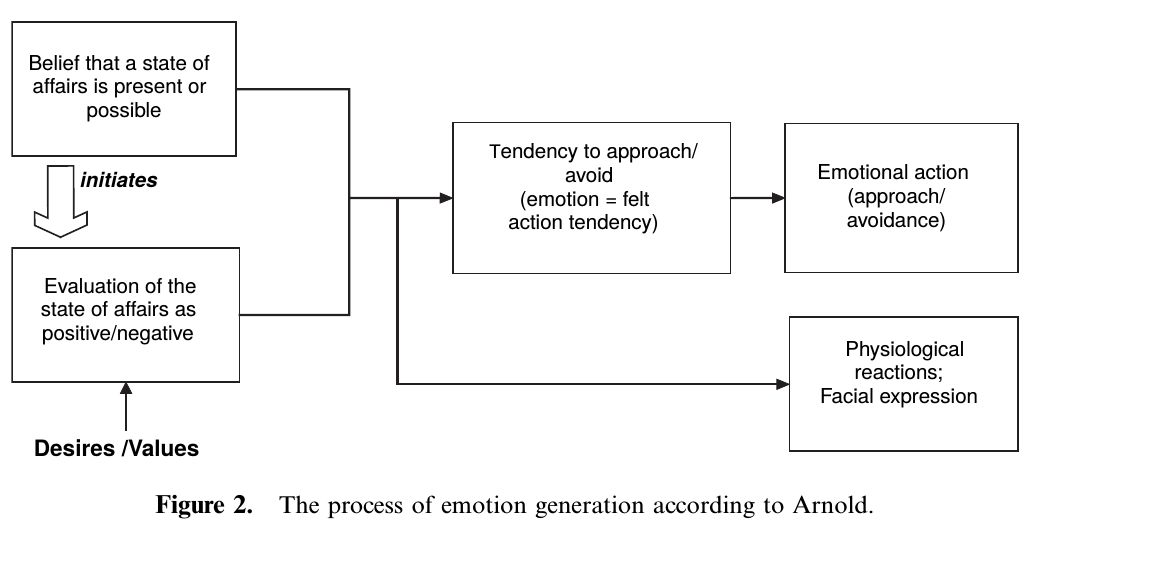
\includegraphics[width=0.8\textwidth]{arnold.jpg}
 \caption{\label{fig:procedure} Emotiontheorie arnold.}
\end{figure}

In 1962 veröffentlichte Sylvan Tomkins sein Buch "Affect, Imagery, Consciousness", womit er als Begründer der Basisemotionstheorie gilt. Tomkins beschreibt dabei 9 universelle Emotionen, wobei sechs von ihnen in zwei verschiedenen Steigerungsformen auftreten. Diese sechs Emotionen sind Interesse/ Begeisterung, Vergnügen/ Freude, Überraschung/ Erschrecken, Leid/Qual, Ärger/Wut und Angst/ Grauen. Die letzten sind Scham/ Demütigung und Ekel vor schlechten Geruch/Geschmack. Wie grundlegend in allen Basisemotionstheorien die folgten, hält er diese Emotionen für elementar und universell. Es wird angenommen, dass sie evolutionär geprägt und vererbt werden. Dabei werden diese Emotionen automatisch von Objekten oder 
Ereignissen ausgelöst. Dabei sind die Emotionen sowohl biologisch analog, wobei dies meint dass  alle Emotionen mit dem gleichen Name dieselben Muster im Verhalten, Körperreaktion und Gesichtsausdruck und Erfahrungen verbunden sind. Durch diese gleichen Muster können Menschen in der ganzen Welt einfach und effektive diese Basisemotionen erkennen und verstehen.Sie sind außerdem homogen, weil sie von derselben Ursache ausgelöst werden.\\

Im selben Jahr publizierten Schachter und Singer ihre Emotionstheorie, die auf verschiedene Weise interpretiert wurde. Zum einen als Zwei-Faktoren-Theorie. Wobei eine Emotion maßgeblich von der kognitiven Interpretation einer Situation und dem Arousal abhängt. Durch diesen Zusammenhang mit dem Arousal als körperliche Reaktion wird die Theorie als Neo-Jamesische Theorie bezeichnet und zum anderen aufgrund ihren kognitiven Anteils zu der Appraisal-Theorien. Ein Emotionserlebnis hängt laut Schachter und Singer von drei Faktoren ab:

\begin{enumerate}
\item eine Situation muss emotionsauslösend interpretiert werden
\item es erfolgt eine unspezifische, physiologische Aktivierung
\item dabei muss die emotionale Situation als Ursache für die unspezifische, physiologische Aktivierung interpretiert werden
\end{enumerate}

Die Höhe der physiologischen Aktivierung beeinflusst dabei die Intensität der Emotion. Die Interpretation der Situation beeinflusst dabei die Qualität der Emotion. Allerdings konnten die Experiment und deren Ergebnisse durch Reisenzein nicht oder nur teilweise reproduziert werden. Im Detail wurden folgende Zusammenhänge überprüft:
\begin{itemize}
\item Dämpfung der physiologischen Erregung führt zur Dämpfung des Emotionserlebnisses - konnte nicht nachgewiesen werden

\item Reinterpretation eines Teils der aktuellen Erregung auf eine "neutrale" Ursache führt zu einer Verminderung des Emotionserlebnisses - konnte nicht nachgewiesen werden

\item Erregungsreste aus Situation A führen nach Beendigung bei nachfolgender Situation B zu einer Verstärkung des Gefühlserlebnisses - nachgewiesen Zillmanscher Erregungstransfer
\end{itemize}

Valin konnte sogar nachweisen, dass eine eingebildete Erregung eine emotionale Reaktion hervorrufen konnte. \\










%Mit diesen zwei Richtungen Appraisal- und Basisemotionstheorien wurden bis 2009 alle Theorien eingeordnet. allerdings gibt es laut Gendron und Barett, welche die historische Einordnung der Emotionstheorien neu rekonstruierten und dabei eine weitere Strömung die psychologisch konstruktivistischen Emotionstheorien definierten.
%Basierend auf der Zwei-Faktoren-Theorie von Schachter und Singer, welche laut ihnen einen Apraisal- Basisemotionen Dualismus aufweist, haben sie unter Einbeziehung vernachlässigter Emotionsarbeiten aus den Dunkelalter der Emotionen den Psychologischen Konstruktivismus konstruiert.





%Im Kern sagt Tomkins’ Affekttheorie, dass alle Menschen exakt neun unterschiedliche Affekte besitzen, die genetisch programmiert und nicht kulturell erworben sind. Die am frühesten entwickelten sechs davon werden von Tomkins als zweistufig beschrieben, wobei die zweite Stufe eine Steigerung der ersten Stufe darstellt: Interesse/Begeisterung, Vergnügen/Freude, Überraschung/Erschrecken, Leid/Qual, Ärger/Wut und Angst/Grauen. Ein weiteres Paar ist entwicklungsgeschichtlich jünger: Scham/Demütigung. Die letzten zwei sind Ekel vor schlechtem Geruch (Tomkins erfand dafür das Wort dismell) und Ekel vor schlechtem Geschmack. Tomkins sieht diese neun Affekte als diskret und elementar an, im Gegensatz zu Emotionen, die komplex und zusammengesetzt sind. Die Affekte des Menschen sind s.E. verwandt mit denen höherer Tiere und nicht zu verwechseln mit den Trieben nach Sigmund Freud. (Siehe auch Abschnitt Affekttheorie im Hauptartikel Psychoanalyse)

%Nach Tomkins und seinem Schüler Paul Ekman gibt es charakteristische und global universelle Gesichtsausdrücke für die Affekte.[7] Die Tatsache, dass selbst blind geborene Kinder diese charakteristischen Gesichtsausdrücke zeigen, wird als Beweis für die angeborene Natur der Affekte angeführt.


%Zur Anfangszeit der institutionalisierten Psychologie (im letzten Drittel des 19. Jahrhunderts) hat man sich zwar recht intensiv mit den Emotionen befasst. Die Psychologie verstand sich damals als Wissenschaft von den Bewusstseinszuständen und Emotionen manifestieren sich zweifellos (zumindest unter anderem) im Erleben. Nach dem Aufkommen des Behaviorismus (um 1915) und der damit verbundenen, vorübergehenden Neudefinition der Psychologie als »Wissenschaft vom Verhalten« wurden die Emotionen allerdings zunehmend vernachlässigt. Im Jahre 1933 sagte der amerikanische Behaviorist Max F. Meyer sogar vorher, die wissenschaftliche Psychologie würde die Beschäftigung mit Emotionen spätestens 1950 als eine Kuriosität vergangener Zeiten belächeln (Meyer, 1933). Statt dessen erlebte die wissenschaftliche Psychologie in den 1950er Jahren jedoch den Niedergang des Behaviorismus. Aber auch die dem Behaviorismus nachfolgende, am Modell der Informationsverarbeitung in Computern orientierte Kognitive Psychologie hat die Emotionen zunächst vernachlässigt. Zum Teil glaubte man, wie schon vorher Meyer (1933), die Kategorie »Emotion« würde sich in nichtemotionale Kategorien auflösen lassen, wie zum Beispiel die Kategorien »körperliche Aktivierung« und »Kognition« (Mandler, 1984; Schachter, 1964). Es spricht jedoch vieles dafür, dass eine Reduktion von Emotionen auf nichtemotionale Zustände nicht möglich ist. Ein zweiter Grund für die Renaissance der Emotionsforschung ist, dass es in den letzten 30 Jahren zu einer Neubewertung der Adaptivität von Emotionen gekommen ist. Traditionell herrschte in der Psychologie und auch in anderen Humanwissenschaften die Ansicht vor, die Emotionen seien Überbleibsel der evolutionären Vergangenheit des Menschen, die zumindest in der modernen Gesellschaft wenig Nutzen hätten (vgl. Arnold, 1960). Was den Menschen nach dieser Sicht auszeichnet, ist sein Verstand, seine Fähigkeit zum vernünftigen Denken und Entscheiden. Dabei seien die Emotionen – als angebliche Produkte primitiver, in archaischen Hirnregionen beheimateter Affektprogramme – nur störend: Sie beeinträchtigen das vernünftige Denken und führen als Folge davon zu Handlungen, die den eigenen besten Interessen der Person zuwiderlaufen. Aus dieser Perspektive gesehen mag die Erforschung der Emotionen nur zu dem Grad wichtig erscheinen, als sie uns in die Lage versetzt, unsere Emotionen besser in den Griff zu bekommen (vgl. Gross, 2008). In den letzten dreißig Jahren hat sich dagegen zunehmend die – historisch freilich nicht wirklich neue (z.B. McDougall, 1908/1960; Meinong, 1894) – Auffassung durchgesetzt, dass Emotionen, auch wenn sie ohne Zweifel manchmal schädliche Effekte haben, insgesamt adaptiv sind (Feldman Barrett u. Salovey, 2002; Frijda, 1994; s. dazu auch Reisenzein u. Horstmann, 2006). Nach Ansicht einiger Forscher sind Emotionen sogar unverzichtbar für adaptives Handeln (z.B. Damasio, 1994). Zumindest aber wird heute in der Psychologie und zunehmend auch in anderen Humanwissenschaften die alltagspsychologische Erkenntnis akzeptiert, dass Emotionen in der »psychischen Maschinerie« eine wichtige Rolle spielen und dass man deshalb ohne die Berücksichtigung der Emotionen nicht ausreichend verstehen kann, wie Menschen »funktionieren«, das heißt, weshalb sie so denken und handeln, wie sie es tun.
V
\section{Biologisch}
Die Emotion als kognitiver Prozess ist ein wichtiger Bestandteil unseres Lebens. Es gibt
ein facettenreiches Spektrum an Emotionen zum Beispiel Angst, Neid, Freude, Wohl-
befinden, Ärger, Wut und viele andere, welche das Handeln und Verhalten der Menschen
beeinflussen. So ist das Ziel eines Menschen ein glückliches, erfülltes Leben zuführen und
Gefahren für Leib und Seele aus dem Weg zu gehen. Doch „obwohl es vielerlei Emotionen
gibt und diese mit zahlreichen körperlichen Prozessen einhergehen, existiert bisher keine
exakte wissenschaftliche Definition des Begriff Emotion“ (Kandel et al., 1996).
Welchen Einfluss Emotionen auf den Menschen und dessen Verhalten haben wurde in
vielen Studien untersucht. Peters et al. (2006) differenzierte in seiner Studie die ver-
schiedenen Rollen, die Emotionen spielen, wenn Menschen Entscheidungen treffen. Er
publizierte, dass Emotionen zu Informationen führen und einen selektiven Fokus für die
Aufmerksamkeit setzen können. Zudem kann eine Emotion als Motivator fungieren und
eine Bewertung alternativer Verhaltensmöglichkeiten treffen. Dies zeigt, dass die Emotion
innerhalb der Kognition und des Verhaltens eine wichtige und entscheidende Rolle, die

%Abb. 2.1: Darstellung der Zwei-Faktoren-Theorie von Schachter und Singer (1962).

es unerläßlich macht, sich mit den Prinzipien und der Wirkungsweise der emotionalen
Verarbeitung auseinanderzusetzen.
Für die Erforschung von Emotionen gibt es einen Ausgangspunkt, welcher in den Gefüh-
len eines Menschen, die dieser subjektiv und bewusst wahrnimmt, liegt. Die Erforschung
dieser Gefühle wurde im letzten Jahrhundert verstärkt. Demzufolge und durch die Weiter-
entwicklung der Technik erhielt die Interpretation von Emotionen und deren kognitiven
Bedeutung einen andere Sichtweise.
Eine der einflussreichsten Theorien der Emotionsforschung ist die „Zwei-Faktoren-
Theorie“ der Emotionen von Schachter und Singer (1962). Sie definiert drei Faktoren, von
denen eine Emotion beeinflusst wird. Der erste Faktor ist die emotionsauslösende Situati-
on, der zweite Faktor ist die unspezifische, physiologische Aktivierung von Neuronen im
Gehirn und der dritte Faktor ist die Betrachtung der emotionale Situation als Ursache für
die physiologische Aktivierung. Dabei soll die Höhe der physiologischen Aktivierung die
Intensität und Interpretation der Qualität von Emotionen beeinflussen (siehe Abb. 2.1).
(Müsseler und Prinz, 2002)
Mit verbesserten Techniken in der Gehirnforschung und neuen Erkenntnissen in der Neu-
rophysiologie entwickelte LeDoux (2001)auf Grundlage diverser Theorien ein Modell,
welches sowohl kognitive als auch biologische Erkenntnisse zur Entstehung von Emo-
tionen integriert. LeDoux untersuchte die Furchtreaktionen sowie deren Ursprung und
fand heraus, dass die Amygdala, eine kleine Region im Vorderhirn, zentraler Bestandteil
des neuralen System (siehe Abb. 2.2) ist. Die Bedeutung der Amygdala für die Angst-
konditionierung und den damit verbundenen Angstreaktionen wurde in diesen Studien
bewiesen.

%Abb. 2.2: Die Amygdala ist ein zentraler Bestandteil in der Emotionsverarbeitung
%(Brain stories, 2011).

Spätere Forschungen zeigen, dass die Amygdala nicht nur der zentrale Bestandteil im
System der Angstverarbeitung ist, sondern auch andere emotionale Verarbeitungssysteme
diese als zentrale Verarbeitungsstation besitzen (Everitt et al., 2000). Ein solches Ver-
arbeitungssystem wird auch Basisnetzwerk der Emotionen bezeichnet. Panksepp (2010)
definiert in einer Studie über Depressionen sechs Kriterien für diese Basisnetzwerke:
\begin{itemize}
\item Sie generieren charakteristische instinktive Verhaltensmuster.
\item Sie werden durch eine begrenztes Set von unkonditionierten Stimuli aktiviert.
\item Die resultierenden Erregungen überdauern herbeigeführte Umstände.
\item Emotionale Erregungen verknüpfen beziehungsweise regulieren verschiedene sen-
sorische Eingaben im Gehirn.
\item Sie kontrollieren das Lernen und helfen höhere Gehirnfunktionen zu realisieren.
\item Höhere Gehirnareale können emotionale Erregungen regulieren.
\end{itemize}

Emotionen dieser Verarbeitungssysteme unterscheiden sich sowohl in der Intensität,
Komplexität als auch in den beteiligten Gehirnarealen. Deshalb werden Emotionen an-
hand ihrer Eigenschaften verschiedenen Begriffen zugeordnet. So werden kurze und star-
ke Emotionszustände, die starke Verhaltenstendenzen besitzen Affekte genannt. Als Emo-
tion werden bewertende Stellungnahmen zu Umweltereignissen, welche der Koordination
von verschiedenen physischen und psychischen Teilsystemen bedürfen, bezeichnet. Im
Gegensatz zu Emotionen werden emotionale Zustände von geringerer Intensivität, länge-
rer Dauer mit einem Fehlen der Objektbezogenheit als Stimmungen definiert. Ein Gefühl

%Abb. 2.3: In der sogenannten Skinnerbox werden Experimente der Angstkonditionierung
%durchgeführt (Ricker, 2011).

wiederum bezeichnet die erlebnisbezogene Seite einer Emotion, zum Beispiel Wut oder
Angst. (Müsseler und Prinz, 2002)
Doch Emotionen können nicht nur anhand ihrer Eigenschaften unterschiedlich katego-
risiert werden sondern auch anhand ihrer prozeduralen Verarbeitung. Panksepp (2010)
unterteilt in diesem Zusammenhang die emotionalen Prozesse in drei Klassen. Affekte
werden im primären Prozess verarbeitet. Sie bezeichnen Urinstinkte, wie Fluchtreflexe
und Angstreaktionen, die genetisch vererbt werden. Affekte sind unkonditionierte Re-
aktionen des Emotionssystems. Sekundäre Prozesse sind erlernte einfache Emotionen,
die das Individuum durch klassisches oder operantes Konditionieren (siehe auch Kapitel
2.5) erwerben kann (Müsseler und Prinz, 2002). Emotionen, die ein vielschichtigeres
Denken und Planen erfordern werden dem tertiären Prozess zugeordnet. Diese Emotio-
nen werden reflektiert und reguliert, außerdem tritt diese Art von Emotionen nur beim
Menschen auf. Die Grundlagen des menschlichen Lebens bilden die primären Prozesse.
Ein neurochemisches Ungleichgewicht in der emotionalen Verarbeitung dieser Prozesse
kann zu einer psychiatrischen Auffälligkeit führen, da die dynamischen sekundären und
tertiären Prozesse mit dem System der primären Prozesse verbunden sind. Es wird also
davon ausgegangen, dass diverse höhere psychologische Funktionen auf der Verarbeitung
einfacher emotionaler Reaktionen beruhen. (Panksepp, 2010)

%Abb. 2.4: Die Darstellung veranschaulicht die zwei Verarbeitungspfade zur Amygdala
%(LeDoux, 2001).

% 2.5 Konditionierung
% Konditionierung bezeichnet einen Lernprozess, welcher bei Menschen und Tieren beob-
% achtet werden kann. Dabei bezeichnet „ Lernen [...] ein(en) Prozess, der als Ergebnis von
% Erfahrungen relativ langfristige Änderungen im Verhaltenpotenzial erzeugt“ (Definition
% Müsseler und Prinz (2002)).
% Es gibt das klassische Konditionieren, welches unkonditionierte Stimuli (US) mit neutra-
% len, konditionierte Stimuli (CS) paart. Voraussetzung eines solchen Lernprozess ist, dass
% der US (z.B. Futter) und der CS (z.B. ein Lichtsignal) mehrmals gemeinsam repräsentiert
% wird. (Müsseler und Prinz, 2002)
% Im Gegensatz zum klassischen Konditionieren beinhaltet das operante Konditionieren
% nicht nur einen Reaktion auf einen Reiz, sondern ein (instrumentelles) Verhalten, dass
% ein Ereignis in der Umwelt herbeiführt (z.B. das Betätigen eines Hebels zum Öffnen
% einer Futterdose). Diese Ereignis würde ohne das Verhalten des Versuchsobjektes nicht
% eintreten. (Müsseler und Prinz, 2002)
\subsection{ Amygdala}
In der Angstkonditionierung wird ein Tier, zum Beispiel eine Ratte, innerhalb eines Ver-
suchsfeldes platziert (siehe Abbildung 2.3). Anschließend wird zuerst ein Ton repräsentiert 


%Abb. 2.5: Forschungen zur Funktion des Hypothalamus.
und kurze Zeit später ein elektrischer Schlag ausgelöst, der eine Angstreaktion
hervorruft. Nach mehreren Wiederholungen, löst allein der Ton eine Furchtreaktion bei
der Ratte aus. Diese und ähnliche Experimenten der Angstkonditionierung zeigten, dass
Tiere, die eine Beschädigung der Amygdala besaßen, keine konditionierten Reaktionen
auf die Präsentation des Tons entwickelten. Es wurde somit bewiesen, dass die Amygdala
als Steuereinheit der Angstreaktionen fungiert. (LeDoux, 2001)
Die entwickelten Furchtreaktionen können je nach Situation und Ausgangszustand so-
wohl bewusst als auch unbewusst stattfinden. Je nachdem, von welchem der beiden Ver-
arbeitungspfade zur Amygdala diese generiert werden. LeDoux nannte diese zwei Wege,
zum Einen den „hohen“ Pfad, welcher vom sensorischen Thalamus über den sensorischen
Kortex zur Amygdala führt und zum Anderen den „niederen“ Pfad, welcher Eingaben
vom sensorischen Thalamus direkt an die Amygdala projiziert (siehe Abb. 2.4). Ein
emotionalerer Reiz wird demzufolge zunächst vom sensorischen Thalamus verarbeitet.
Bestandteile des sensorischen Thalamus sind zum Beispiel der Visuelle oder Rhinale
Kortex, welche visuelle beziehungsweise geschmackliche Eingaben verarbeiten. Diese
Informationen können anschließend auf dem kürzeren und direkten Weg an die Amygdala
weitergegeben werden, wobei die Repräsentation des Reizes innerhalb dieses Verarbei-
tungspfades eher rudimentär und grob ist. Desweiteren kann die Informationsweiterlei-
tung an die indirekte Bahn über den sensorischen Kortex erfolgen. Dieser Pfad liefert
eine genaue aber auch langsamere Repräsentation des Reizes. Durch die Verarbeitung in
höheren Gehirnarealen werden Objekte erkannt, eingeordnet und die aktuelle Situation
analysiert. Am Beispiel einer Gefahrensituation ermöglicht die direkte Bahn ein beson-
ders schnelles, reflexartiges Handeln (wie ansteigende Herzfrequenz, Adrenalinausstoss,

%Abb. 2.6: Im Zwischenhirn befindet sich der Hypothalamus, der eine sehr starke Verbin-
%dung zur Amygdala besitzt (Focalaxis, 2011).

Weglaufen) und die indirekte Bahn die Bewertung und Analyse der Situation (Erkennen
was ist die Gefahr, wie gefährlich ist die Situation). (LeDoux, 2001)
\subsection{ Hypothalamus}
Die Amygdala spielt neben der Angstkonditionierung auch eine wichtige Rolle beim Ler-
nen durch positive und appetitive (d.h. belohnenden) Ereignisse. Dies bewiesen Nakamura
et al. (1987) in Experimenten, die eine Verabreichung von verschiedenen Nahrungsmitteln
als Belohnung verwendeten. In diesen Studien zeigten sie, dass besonders die Verbin-
dung von Amygdala und Hypothalamus für das Gefühl von Hunger und Sättigung einer
Nahrung von Bedeutung ist. Während des Experimentes wurden Neuronen des Lateralen
Hypothalamus von Ratten abgeleitet und deren Aktivität aufgezeichnet(siehe Abb. 2.5a).
Es wurden verschiedene Gerüche, wie Orange oder Traube als positiven CS eingesetzt.
Zudem fundierte ein Schlag oder Kneifen in den Schwanz als negativer CS. Durch Prä-
sentation der entsprechenden CS erfolgte das Konditionieren der Ratte, sodass diese beim
Auftreten des entsprechenden Reizes die verabreichte Glukoselösung zu sich nahm.
Der Lernprozess mit einem appetitiven Stimulus kann vereinfacht, wie in Abb. 2.5b,
dargestellt werden. Ein beliebiger Stimulus wird mit einer primären Belohnung (Futter

%Abb. 2.7: Experimenteller Aufbau zur Dopaminausschüttung. Links der Versuchsaufbau
%und rechts die Aktivität der Dopaminzelle (Schultz et al., 1998).

oder Wasser) durch ständige Wiederholung konditioniert. Der konditionierte Stimulus
löst durch die Erwartung einer Belohnung einen internen angeregten Zustand aus. Meist
korrespondiert diese Erwartung mit Hunger oder Durst. Als Folge der Erwartungshaltung
erfolgt anschließend die Verhaltensreaktion, das heißt Enttäuschung bei Ausbleiben und
Zufriedenheit bei Belohnungsvergabe. Nach Nakamura et al., werden diese internen Zu-
stände durch den lateralen Hypothalamus gesteuert, denn Neuronen dieses Gehirnareals
reagierten selektiv auf die verschiedenen konditionierten Stimuli.
Die Reaktionen der Ratte, zum Beispiel Hunger, Durst oder Blutdruckänderungen, er-
klären sich aus der Funktion des Hypothalamus. Dieser befindet sich im Zwischenhirn,
dargestellt in Abbildung 2.6 und steuert die vegetativen Funktionen des Gehirns, un-
ter anderem die Aufrechterhaltung von Temperatur, Blutdruck und Osmolarität, die zur
Homöostasie zusammengefasst werden, oder die Regulation der Nahrungs- und Wasser-
aufnahme. Zusätzlich veranlasst der Hypothalamus die Bildung von sogenannte Effekt-
hormonen, wie Dopamin, welche bei Lernaufgaben und der Konditionierung ein zentrale
Aufgabe besitzt.
\subsection{ Basalganglien}
Der Dopaminhaushalt, der sich während eines Lernprozesses ändert, wird durch die
Basalganglien reguliert (Schultz et al., 1998). Um die Ausschüttung und Senkung von
Effekthormonen insbesondere von Dopaminen zu erklären, führten Schultz et al. in ihrer
Studie eine Verhaltensaufgabe durch (siehe Abb.2.7). In diesem Experiment löste das Tier
16

%Abb. 2.8: Darstellung der Basalganglien und ihren dazugehörigen Gehirnarealen (The
%Dana Fondation, 2011).
in einem selbst gewählten Moment einen berührungsempfindlichen Schalter aus und griff
in die Futterbox, um daraus ein Stückchen verstecktes Futter einzusammeln. Die Erregung
der Dopaminzelle, nachdem das Tier in die Futterbox gegriffen hat, ist in Abbildung 2.7
dargestellt. Der Movement-onset bezeichnet den Moment indem das Tier den Schalter
bewegt hat.
In diesem Zusammenhang fanden Schultz et al. heraus, dass die Basalganglien Dopamine
nicht nur regulieren sondern auch einen Fehler in der Vorhersage von Belohnungen ko-
dieren. Eine Belohnungsvorhersage erfolgt durch die Aktivität der Dopaminneurone wäh-
rend der Präsentation des CS. Erfolgte nach dieser Präsentation eine Belohnung, initierten
die Neuronen der Basalganglien einen Dopaminausstoß. Wurde jedoch die Belohnung
ausgelassen, reagierten die Zellen mit einer Senkung des Dopamins. Diese Senkung stellt
die Detektion des Fehlers in der Belohnungsvorhersage dar.
2.5.4 Orbitofrontaler Kortex
Neuronen in den Basalganglien können zwar Belohnungsvorhersagen treffen, jedoch kön-
nen sie nicht zwischen den verschiedenen Belohnungen (aversiv oder appetitiv) unter-
scheiden. Aus diesem Grund untersuchten Schultz et al., in welchem Gehirnareal eine
solche Verarbeitung stattfindet. Hier wurden sie im Orbitofrontalen Kortex fündig. Bei
Tests mit unterschiedlichen Belohnungen zeigten 70% der gemessenen Neuronen eine
korrespondierende Antwort. Sie antworteten entweder bevorzugt auf die eine oder auf
die andere Belohnung. Daraus lässt sich schließen, dass diese Neuronen Details von Be-
lohnungen kodieren. Verbindungen mit dem sensorischen Thalamus und der Amygdala
ermöglichen dieser Hirnregion eine subjektive Wertebildung für Objekte. Die Übertra-
gung einer solchen Wertigkeit erfolgt unter anderen an die Basalganglien, in welchen
anschließend entschlüsselt wird ob ein positiver oder negativer Reiz vorliegt und die Do-
paminausschüttung oder Dopaminsenkung unterdrückt oder veranlasst werden kann.
\subsection{Künstlichen Intelligenz und Robotik}

\thispagestyle{empty}
\chapter{Exisitierende Emotionsmodelle}

Für die Simulation menschlicher Emotionen existieren in der Literatur viele Emotionsmodelle, die das
emotionale Verhalten von Menschen erklären bzw. simulieren soll (Marsella and Gratch, 2010). Die
Modelle sind unterschiedlich komplex und verfolgen unterschiedliche theoretische Ansätze der
Psychologie (Marsella and Gratch, 2014). Allerdings sind wenige dieser Modelle mit realen Messdaten
aus psychologischen Experimenten validiert worden (Marinier et al., 2013). Das in der Dissertation
entwickelte Emotionsmodell soll sowohl den Anspruch der theoretischen Fundiertheit in der
Psychologie als auch deren funktionale Korrektheit mit Hilfe realer Experimentdaten nachweisen
können.
\thispagestyle{empty}
\chapter{Emotionsmodell innerhalb einer Mensch-Simulation}
\section{Projektkontext}
\section{Theoretische Grundlagen}
\section{Modellierung}
\section{Ergebnisse}
\section{Fazit}

\thispagestyle{empty}
\chapter{Experimenteller Aufbau und Validierung des eigens entwickelten Computermodells der Emotionen}
 \section{Aufbau und Validierung Emotionsmodell "Barcelona"-Modell}
 \section{Validierung und Erweiterung des Modells anhand eines weiteren Experimentes}

\thispagestyle{empty}
\chapter{Zusammenfassung}

Zusammenfassend ist zu sagen:

Das nichts passiert ist bisher. OK das ist erstmal schwierig zu belegen aber daß wird schon gehen. Ohoh das tipper von längeren Texten könnte schon schwieriger werden. ES scheint nicht so einfach wie gedacht aber voll muss man sich nur noch dran gewöhnen. ES wird bestimmt mit der zeIchtT besser weil man die Tasten bessehr trifft manchmal dauert das erscheinen der Buchstaben aber lange...  Ich hab die Aktualisierung nun ausgeschaltet und es geht um einiges besser!!!  

Jetzt gehat es eventuell besser? Irgendwie schon aber wer weiß wie lange? Scheint ja immer nur ein paar sekungen so zu gehen. Oder etja doch länger.  ICh scheine die Fr Taste immer zu drükken. ICh musß mehrüber die Ästen fliegen.  UNdmeine Hand nicht auf der tastTür liegen lassen.  Dann geht  esdoch etwas besser. ICh hoffe das wird noch mit der zeit. DA hilft nur üben üben üben. Ohhh man das ist schon etwas anstrengend...Vor allem die Korrektur!!! Wenn mann innerhalb eines wortes etwas ändern möchte.... UNd die Leertaste treffe ich auch manchmal nicht und hier bin ich wieder. Es ist wirklich nicht so einfach.  Ich hoffe das gibt sich.  Ich bete inständig dass es so sein wird...Manchmal ist der Mauszeiger einfach irgendwo anders... Ok weiter im Text.  Also wir haben uns ja immer gefragt was man daraus machen könnte. 
Ohje das mit dem anzeigen wird auch schwierig... 

Die frage ist warum. Irgendwie macht er nach jedem Zeichen eine Leerzeile weg und daNN sehe ich nicht mehr was ich schreibe. Das ist Mist !!!!!! OK ihr hier nochmal... Und nun?? Wie soll ich damit umgehen??? Und nun was soll ich dmit machen??? Das ist sehr nervig... Dass es nach und nach die leerzeilen löscht... Das macht so doch keinen Spaß... 


nochmal ohhh das sieht schon besser aus. aber jetzt gibt es keine groß- und kleinschreibung mehr. ok also hier nochmal die andere tastatur. jetzt habe ich gar keine veränderung mehr....
Ok nochmal und wenn ich das hier nich will.
 das 
 
 AsAs nicht!!!!!!! Das  i
 
  die das  und nun geht wieder alles ... aber ohne korrektur. Naja dann muss es eben so gehen. Geht ja sonst so auch. hallo hier bin ich. und das ist gut so... :) ach naja ohne rechtschreibprüfung geht es ja schon viel besser. 
 
 
 
 Ok   hire nochal ist dash auvh so dad gehha aufksbr
 IRgendwie das scheie hsllo gehnicht bedstrt dsd t das uuss foch besser errnrn. WarJm isdad ssirgn keine ahnungn wordasn liegt.
 Aber schneint die eingsbe besser zu laufen. oder auch nicht. ich hab keine ahnung warum das jetzt ausgeschalten ist.... ok hier sind wir nun bei googles tastatur und es erscheint keine. irgendwie hat das mit den einstellungen nich hin.
 test ohhh keine rechtschreibung mehr. ok das ist auch besser so. weil es eh nicht funktioniert hier.
 
 
 
 
 
 
 
 
\thispagestyle{empty}


%----------------------------------------------------------------------------------------
%	Anhang
%----------------------------------------------------------------------------------------

\addtocontents{toc}{\vspace{2em}} % Platzhalter nach vor toc

\appendix % Erstellen des Anhangs

%  Einbinden aller Dateien aus dem Ordner Anhang

\chapter{Lineare Algebra}

Hier.
\thispagestyle{empty}
%\include{Apendices/AppendixB}
%\include{Apendices/AppendixC}

\addtocontents{toc}{\vspace{2em}} % Platz nach toc


%----------------------------------------------------------------------------------------
%	Bibliografie
%----------------------------------------------------------------------------------------
\backmatter
\nocite{*}
\bibliographystyle{plain}
\bibliography{LiteraturDiss.bib} %Name der .bib Datei






\end{document}